\documentclass[]{report}

% Packages and commands file
\input{include/packagescommands}
\usepackage{amsmath}
% Settings (Metadata)
\input{include/settings}

%definitions
\input{include/definitions}



\begin{document}
% Titlepage
% Chalmers title page
\begin{titlepage}

\AddToShipoutPicture{\backgroundpic{-4}{56.7}{figures/frontpage}}
\mbox{}
\vfill
\addtolength{\voffset}{2cm}
\begin{flushleft}
	{\noindent {\Huge Finding the Jeffrey Orbits} \\[0.5cm]
	\emph{\Large Master's Thesis in Complex Adaptive Systems} \\[.8cm]
	
	{\huge Staffan Ankardal}\\[.8cm]
	
	{\Large Department of Physics \& Engineering Physics \\
	Non-linear Dynamics \& Statistical Physics \\
	\textsc{Chalmers University of Technology} \\
	Gothenburg, Sweden 2011 \\
	Master's Thesis 2011:1\\
	} 
	}
\end{flushleft}

\end{titlepage}
\ClearShipoutPicture
% End Chalmers title page



% % TEMPORARY DOUBLE SPACIN % %
\doublespacing

% Abstract
\input{abstract.tex}

% Table of contents
\newpage
\pagenumbering{roman}
\setcounter{page}{1}
\pagestyle{fancy}
\setspecialhdr
\tableofcontents


% Main area
\newpage
\setdefaulthdr
\pagenumbering{arabic}	
\setcounter{page}{1}

\chapter{Introduction}
\section{Introduction}
My goal in this thesis is to study and better understand the dynamics of ellipsoidal particles in shear flows. The thesis is a continuation of two previous MSc theses\cite{AntonThesis, JonasThesis}. The methodology is to experimentally measure the orientational dynamics of micrometer length glass particles in a shear flow and comparing the results to those of theoretical models. In the first part of the thesis I describe the improvements that were made to the experimental setup, most importantly an automated tracking. In the second part of the thesis the measurements and their analysis is discussed. But before discussing either of these subjects more in depth some background and theory is needed.

\subsection{Background}
Understanding the orientational dynamics of particles in flow might appear somewhat esoteric to someone unfamiliar with the field, but there is a number of topics where it is very useful. In medical applications understanding the dynamics of ellipsoidal particles such as bacteria can be relevant to a detailed understanding of their interactions with cells and other bodies. This is discussed by Tolga \emph{et al}~\cite{Tolga}. 

One of the most influential papers in the study of particle dynamics in flow was by Einstein in 1905~\cite{Einstein}. He showed how much suspended spherical particles would increase the viscosity of a fluid. Jeffery in his 1922 paper~\cite{Jeffery} extended these results to ellipsoidal  particles and derived equations for the orientational dynamics of axisymmetric particles, in other words how the particles would rotate as a function of time. For systems where inertial effects could be disregarded the motion was found to be periodic and depending only on the initial condition of the particle. 

Investigation of triaxial particles was started by Gierszewski \& Chaffey~\cite{Chaffey} and was continued by Hinch \& Leal~\cite{Leal} and more recently by Yarin \emph{et al}~\cite{Yarin}. 
The dynamics Jeffery had found for axisymmetric particles were periodic, but it was shown by Hinch \& Leal that for triaxial particles some orbits would be doubly periodic, in other words following two separate independent periods. This behaviour will in this thesis be referred to as \emph{quasi-periodic}.

Yarin \emph{et al} used numerical simulations to generate a surface of section~\cite{SurfaceOfSection} for ellipsoidal particles with different shapes. They showed that not only were there double periodic or quasi periodic orbits but when the particles were sufficiently different from axisymmetric there would be chaotic orbits. 
Several other surfaces of section were produced by Johansson ~\cite{AntonThesis} using the same method as Yarin. It was shown that even small asymmetries of the order of 1\% lead to quasi-periodic motion for some initial conditions.

Attempts to experimentally verify these theoretical results were initially performed by Goldsmith and Mason in 1962~\cite{Mason} who used flow in a glass pipe to observe the rotation rate for several different particle shapes. They confirmed that the rotation rate matched well with that predicted from Jeffery orbits but they did not study the actual orbits. Since then most experimental research, such that as by Harlen and Koch~\cite{fibersspension} has focused on how diluted suspensions of particles affect the properties of a liquid. Only tangential efforts such as by Tolga~\cite{Tolga} were concerned with the Jeffery orbits. A good summary of both theoretical and experimental results was written by Petrie~\cite{Petrie} in 1999.

The first dedicated experiments to measure the actual Jeffery orbits in angular components and verify the orientational dynamics were performed by Einarsson \emph{et al}~\cite{JonasExperiment}. Although there were some promising results, the vast majority of particles were asymmetric to the degree that their orbits were chaotic or highly quasi-periodic. Moreover the width and length of particles varied greatly and could not be measured accurately.
This meant that although the orbits could be qualitatively shown to be similar to some 
Jeffery orbits, no particular particle could be shown to exhibit both quasi periodic and periodic motion. No particle could also be well matched to a particular orbit, but different particles could be shown to be qualitatively simililar to different types of orbits. There was also few particles that very closely retraced its trajectory along the entire length of the channel when the flow was reversed, which indicates that their deviation from periodic motion was not caused by noise, as that would not be reversible.


% I really want a cite for thus but how could I possibly do that.
The goal of this thesis is to experimentally verify the results of Yarin and Hinch, Leal\cite{Yarin, Leal} and show that the same particle will show different types of motion for different initial conditions. Furthermore that different particles will show different motion for the same initial conditions based on the asymmetry. This is done by observing the orientation of a micrometer length particle in a creeping shear flow. The flow is shown to be creeping by demonstrating that the particle dynamics revert as the flow is reverted. The results are then will then be compared to theoretical predictions for different initial conditions and asymmetries.

%doing so would be very important to actually motivating using these results as well as possibly finding the limitations of this theory in real world applications. Understanding the dynamics of ellipsoidal particles in shear flow could be useful for example in our understanding of microscopic bacteria in blood stream 


\chapter{Theory}
\section{Introduction}
My goal in this thesis is to study and better understand the dynamics of ellipsoidal particles in shear flows. The thesis is a continuation of two previous MSc theses\cite{AntonThesis, JonasThesis}. The methodology is to experimentally measure the orientational dynamics of micrometer length glass particles in a shear flow and comparing the results to those of theoretical models. In the first part of the thesis I describe the improvements that were made to the experimental setup, most importantly an automated tracking. In the second part of the thesis the measurements and their analysis is discussed. But before discussing either of these subjects more in depth some background and theory is needed.

\subsection{Background}
Understanding the orientational dynamics of particles in flow might appear somewhat esoteric to someone unfamiliar with the field, but there is a number of topics where it is very useful. In medical applications understanding the dynamics of ellipsoidal particles such as bacteria can be relevant to a detailed understanding of their interactions with cells and other bodies. This is discussed by Tolga \emph{et al}~\cite{Tolga}. 

One of the most influential papers in the study of particle dynamics in flow was by Einstein in 1905~\cite{Einstein}. He showed how much suspended spherical particles would increase the viscosity of a fluid. Jeffery in his 1922 paper~\cite{Jeffery} extended these results to ellipsoidal  particles and derived equations for the orientational dynamics of axisymmetric particles, in other words how the particles would rotate as a function of time. For systems where inertial effects could be disregarded the motion was found to be periodic and depending only on the initial condition of the particle. 

Investigation of triaxial particles was started by Gierszewski \& Chaffey~\cite{Chaffey} and was continued by Hinch \& Leal~\cite{Leal} and more recently by Yarin \emph{et al}~\cite{Yarin}. 
The dynamics Jeffery had found for axisymmetric particles were periodic, but it was shown by Hinch \& Leal that for triaxial particles some orbits would be doubly periodic, in other words following two separate independent periods. This behaviour will in this thesis be referred to as \emph{quasi-periodic}.

Yarin \emph{et al} used numerical simulations to generate a surface of section~\cite{SurfaceOfSection} for ellipsoidal particles with different shapes. They showed that not only were there double periodic or quasi periodic orbits but when the particles were sufficiently different from axisymmetric there would be chaotic orbits. 
Several other surfaces of section were produced by Johansson ~\cite{AntonThesis} using the same method as Yarin. It was shown that even small asymmetries of the order of 1\% lead to quasi-periodic motion for some initial conditions.

Attempts to experimentally verify these theoretical results were initially performed by Goldsmith and Mason in 1962~\cite{Mason} who used flow in a glass pipe to observe the rotation rate for several different particle shapes. They confirmed that the rotation rate matched well with that predicted from Jeffery orbits but they did not study the actual orbits. Since then most experimental research, such that as by Harlen and Koch~\cite{fibersspension} has focused on how diluted suspensions of particles affect the properties of a liquid. Only tangential efforts such as by Tolga~\cite{Tolga} were concerned with the Jeffery orbits. A good summary of both theoretical and experimental results was written by Petrie~\cite{Petrie} in 1999.

The first dedicated experiments to measure the actual Jeffery orbits in angular components and verify the orientational dynamics were performed by Einarsson \emph{et al}~\cite{JonasExperiment}. Although there were some promising results, the vast majority of particles were asymmetric to the degree that their orbits were chaotic or highly quasi-periodic. Moreover the width and length of particles varied greatly and could not be measured accurately.
This meant that although the orbits could be qualitatively shown to be similar to some 
Jeffery orbits, no particular particle could be shown to exhibit both quasi periodic and periodic motion. No particle could also be well matched to a particular orbit, but different particles could be shown to be qualitatively simililar to different types of orbits. There was also few particles that very closely retraced its trajectory along the entire length of the channel when the flow was reversed, which indicates that their deviation from periodic motion was not caused by noise, as that would not be reversible.


% I really want a cite for thus but how could I possibly do that.
The goal of this thesis is to experimentally verify the results of Yarin and Hinch, Leal\cite{Yarin, Leal} and show that the same particle will show different types of motion for different initial conditions. Furthermore that different particles will show different motion for the same initial conditions based on the asymmetry. This is done by observing the orientation of a micrometer length particle in a creeping shear flow. The flow is shown to be creeping by demonstrating that the particle dynamics revert as the flow is reverted. The results are then will then be compared to theoretical predictions for different initial conditions and asymmetries.

%doing so would be very important to actually motivating using these results as well as possibly finding the limitations of this theory in real world applications. Understanding the dynamics of ellipsoidal particles in shear flow could be useful for example in our understanding of microscopic bacteria in blood stream 
\section{Fluid dynamics}

In order to understand the motivations, limitations and behaviour of the experiment we need to know about a few key concepts in fluid dynamics.

\subsection{Navier Stokes}


\subsection{Reynold's Number}
The Reynolds number (Re) is a dimensionless number describing the ratio of inertial forces to viscous forces in a flow. This is not a very strict definition, but suffices to explain that the Reynolds number can be used to characterize the so called flow regime of a system. 

The two major flow regimes are Laminar flow, where viscous forces dominate over inertial forces, and the turbulent regime where inertial forces dominate. The area where neither is significantly larger is referred to as transitional flow, which may show either chaotic of laminar behaviour. 

A rough characterization of laminar and chaotic flow can be seen in figure \ref{fig:laminar_flow}

\begin{figure}\label{fig:laminar_flow}

\includegraphics{Images/laminarFlow.png}
\end{figure}

The Reynolds number (Re) is defined as \cite{introfluid}

\begin{equation}\label{eq:reynolds}
Re = \frac{U L \rho}{\mu}
\end{equation}

where $U$ is the characteristic velocity, $L$ is the characteristic length, $\rho$ is the density and $\mu$ is the dynamic viscosity. 

As the Reynolds number is a ratio, a flow is predicted to be laminar if $Re << 1$ which is the primary concern in this thesis.

\subsection{Stokes Drag and Stokes's law}
The drag force exerted by a fluid on a spherical particle for $Re << 1$ is found using the so called Stokes's law \cite{introfluid2}

\begin{equation}
F_D = 6\pi \mu R v
\end{equation}
and equating this with the gravitational force acting on the sphere

\begin{equation}
F_G = (\rho_p - rho_l) g\cdot \frac{4\pi R^3}{3}
\end{equation}

the velocity of a steadily sinking sphere is found to be 

\begin{equation}\label{eq:fallingSphere}
v_s = \frac{2}{9} \frac{\Delta \rho}{\mu} g R^2
\end{equation}

% % Remove this when feeling in a more removy mood
In order to approximate the falling velocity of our particles we can make use of Stokes law which describes the drag force on an object in laminar flow, and more specifically in the case of a sphere, 
where $\Delta\rho$ is the difference in density between the sphere and the liquid, $g$ is the specific gravity, $\mu$ is the dynamic viscosity and $R$ is the radius of the sphere.  


% % Ignore these sections for now as they are not needed

\subsection{Shear}

\subsection{P\'{e}clet Number}
The p\'{}clet number describes the ratio of thermal noise to other stuff. I really don't know anything about the piclet number.


\section{Euler angles and coordinate system}
When describing rotating particles it is common to use the so called Euler Angles. These are defined 

DEFINITION OF EULER ANGLES

This is illustrated in figure \ref{fig:eulerangles} where each prim marks one more step of rotation to the coordinate system of

\begin{figure}
\begin{center}
\includegraphics[width=0.7\textwidth]{figures/theory/eulerangles.png}
\end{center}
\caption{The Euler angles illustrated using a series of coordinate rotations. This is the normal way of illustrating the Euler angles as it is how they are defined.}
\label{fig:eulerangles}
\end{figure}


\begin{figure}
\begin{center}
\includegraphics[width=0.7\textwidth]{figures/theory/EulerAngles.png}
\end{center}
\caption{The Euler angles illustrated using an ellipsoid. This alternate visualization shows the angles with a point of view similar to that of the camera in the experiment. Note although $\psi$ has an impact on the particle dynamics, as the particle is nearly axis-symmetric we can not observe it}
\label{fig:eulerparticle}
\end{figure}




\section{Jeffery orbits}
\label{sec:jeffery}
The Jeffery orbits describe the motion of an ellipsoidal particle in Stokes flow. The orbits for axisymmetric ($a_x = a_z \ne a_y$) ellipsoidal particles were found by Jeffery and reformulated by Yarin \emph{et al}~\cite{Yarin} who computed orbits for asymmetric particles. The equations of motion for a triaxial particle in the form of Yarin \emph{et al} is

\begin{subequations}\label{eq:jeffrey}
\begin{align}
\frac{d\theta}{dt} 	&= (g_2 \sin \psi + g_3 \cos \psi ) \sin \theta, \\
\frac{d\phi}{dt} 	&= \tfrac{1}{2} + g_3\sin \psi - g_2 \cos \psi,\\
\frac{d\psi}{dt}	&= g_1 + (g_2\cos \psi - g_3\sin \psi) \cos \theta \\
\end{align}
\end{subequations}

where the functions  $g_i$ are defined as

\begin{subequations}
\begin{align}
g_1 &= \frac{a_y^2 - a_z^2}{2(a_y^2 + a_z^2)} 
		\left(-\tfrac{1}{2}(\cos^2 \theta + 1 )\sin 2\phi \sin 2\psi + \cos\theta \cos 2\phi \cos 2\psi \right), \\
g_2 &= \frac{a_z^2 - a_x^2}{2(a_x^2 + a_z^2)}
		\left( -\cos\theta \sin 2\phi \sin\psi  +  \cos 2\phi \cos\psi \right), \\
g_3 &= \frac{a_x^2 - a_y^2}{2(a_x^2 + a_y^2)}
		\left( \cos\theta \sin 2\phi \cos\psi + \cos 2\phi \sin\psi \right).
\end{align}
\end{subequations}

where $(\phi, \theta, \psi)$ are the Euler angles seen in figure \ref{fig:eulerangles} and . 

Looking at figure \ref{fig:orbitparams} we see that $n_x$ and $n_y$ have periodic orbits, we call each one of these periodic changes a flip. The period of flipping $T$ is for an axisymmetric particle \cite{Jeffery}

\begin{equation}\label{eq:flipRate}
T = 2\pi \left( \lambda + \frac{1}{\lambda} \right)\frac{1}{\kappa},
\end{equation}

\noindent where $\kappa$ is the shear rate. 

Solutions to the equations of motions can be found with numerical methods as shown by Yarin \cite{Yarin}. Note that the eq. \ref{eq:jeffrey} uses the coordinates from Yarin which differ from the ones used in this thesis in the same way as is discusse in Johansson \cite{AntonThesis}. The time evolution of $\theta$ and $\psi$ for different initial conditions can be plotted in a Poincaré map, also known 
as a Surface-of-Section (S.O.S.) \cite{poincare}. This plots the $\psi$ and $\theta$ coordinates each time $\phi = 0$. The points for every initial condition is bound to a certain region of such a map called the orbit. A few such maps are shown in Figure \ref{fig:orbitmaps}

For a particle with an $\epsilon \in \left[0.01-0.05\right]$ there are essentially three classes of orbits based on the initial condition $\theta_0$.

\begin{enumerate}
\item \textbf{Periodic}: $\left|\theta_0\right| \approx 1$ in which there is little variation and the particle is largely periodic with fluctuations too small to measure.
\item \textbf{Quasi-periodic sign preserving}: For $\left|\theta_0\right|> \theta_b$ the amplitude of $\cos(\theta)$ changes noticeably but does not change sign. $\theta_b$ is some breaking point that changes for different $\epsilon$
\item \textbf{Quasi-periodic sign changing}: For small $\left|\theta_0\right|$ the amplitude of $\cos(\theta)$ will change noticeably and change in sign from positive to negative.
\end{enumerate}

For larger asymmetries $\epsilon > 0.05$ there are chaotic orbits that appear as areas with dots. Chaotic orbits can been seen around the quasi-periodic circular orbits in figure \ref{fig:orbitmap4} where they appear as a 'sea' of dots.

Simulations of these three different types of orbits are illustrated in figure \ref{fig:orbittypes} both on the S.O.S. as well as the in components of $\mathbf{n}$ as a function of time. We can see that while $n_x$ and $n_y$ are periodic, albeit with different amplitudes, the 
behaviour of $n_z$ is significantly different. For the $n_z \approx 1$  orbit shown in green it is constant on the S.O.S and is simply periodic over time. For the sign presercing quasi-periodic orbit in red it is bent on the S.O.S and we can see in the time series that it is doubly periodic as it peaks with a fixed period but the amplitude of the peaks vary periodically themselves. For the sign changing quasi-periodic orbit in blue $n_z$ changes sign, again with a fixed period.


%\begin{figure}[H]
%\centering
%\begin{subfigure}[b]{0.45\textwidth}
%\includegraphics[width=0.9\textwidth]{figures/method/channelDetail.pdf}
%\caption{Sketch of the channel}\label{fig:channelsketch}
%\end{subfigure}
%\begin{subfigure}[b]{0.45\textwidth}
%\includegraphics[width=0.9\textwidth]{figures/method/ChannelZoomed.jpg}
%\caption{Picture of the channel}\label{fig:channelpicture}
%\end{subfigure}
%\caption{A sketch of the channel as well as a picture of the channel as it is set up during a measurement. The channel is only 150 $\mu$m deep, but the PDMS surrounding it is around 15 mm to try and prevent the channel from expanding and contracting too much.}
%\label{fig:channel}
%\end{figure}


\begin{figure}[H]
\centering
\begin{subfigure}[b]{0.45\textwidth}
\includegraphics[width=\textwidth]{figures/theory/map.pdf}
\caption{A poincare map}\label{fig:orbitmap}
\end{subfigure}\hspace{1em}%
\begin{subfigure}[b]{0.5\textwidth}
\includegraphics[width=\textwidth]{figures/theory/orbit.pdf}
\caption{The time series for the components \\ of the unit vector.}\label{fig:orbitparams}
\end{subfigure}
\caption{A Poincare map and three different orbits for a simulated particle with $\lambda=7$ and $\epsilon=0.05$. The three orbits highlight the three different kinds of motion, the quasi-periodic sign changing orbit in blue, the quasi-periodic sign preserving orbit in red and the periodic orbit in green. We see that while $n_x$ and $n_y$ look qualitatively similar but differ in amplitude for the different orbits, $n_z$ shows three different types of behaviour}
\label{fig:orbittypes}
\end{figure}



\begin{figure}[H]
\centering
\begin{subfigure}[3a]{0.40\textwidth}
\includegraphics[width=\textwidth]{figures/theory/7-1-1.pdf}
\caption{Poincare map for $\lambda = 7, \epsilon = 0$.}\label{fig:orbitmap1}
\end{subfigure}\hspace{1em}%
\begin{subfigure}[3b]{0.40\textwidth}
\includegraphics[width=\textwidth]{figures/theory/7-1o01-1.pdf}
\caption{Poincare map for $\lambda = 7, \epsilon = 0.01$.}\label{fig:orbitmap2}
\end{subfigure} \\
\begin{subfigure}[3a]{0.40\textwidth}
\includegraphics[width=\textwidth]{figures/theory/7-1o05-1.pdf}
\caption{Poincare map for $\lambda = 7, \epsilon = 0.05$.}\label{fig:orbitmap3}
\end{subfigure}\hspace{1em}%
	\begin{subfigure}[3b]{0.40\textwidth}
\includegraphics[width=\textwidth]{figures/theory/7-1o25-1.pdf}
\caption{Poincare map for $\lambda = 7, \epsilon = 0.25$.}\label{fig:orbitmap4}
\end{subfigure} 
\caption{Four Poincare maps for different $\epsilon$. Already at $\epsilon = 0.01$ there are noticeably quasi-periodic 
orbits around the centre at $\cos(\theta) \approx \psi \approx 0$ but it is also a significantly larger region for $\epsilon = 0.05$. For $\epsilon = 0.25$ we can see chaotic orbits surrounding the circular orbits in the centre that appear as a 'sea' of dots. Note that some wavelike pattern can appear to exist in the figure \ref{fig:orbitmap2} and  \ref{fig:orbitmap2}, this is caused by aliasing/compression issues with printing several curved lines close together.}\label{fig:orbitmaps}
\end{figure}

\subsection{Winding number} \label{sec:winding}
The quasi-periodic orbits are also referred to as double-periodic~\cite{Yarin}. This to emphasize the fact that the amplitude of the short period $\theta_2$ also varies periodically with period $\theta_1$. The ratio between the two periods is referred to as the winding number $\omega$

\begin{equation}\label{eq:winding}
\omega = \frac{\theta_1}{\theta_2}.
\end{equation}

\noindent The winding number of the quasi-periodic sign preserving orbit from figure \ref{fig:orbittypes} is illustrated in Figure \ref{fig:windingDef}.

\begin{figure}[H]
\begin{center}
\includegraphics[width=0.7\textwidth]{figures/theory/WindingNrFixed2.pdf}
\end{center}
\caption{The $n_z$ sign preserving quasi-periodic orbit from figure \ref{fig:orbitparams} over a longer time, highlighting the short period $\theta_2$ which is simply the period of $\phi$ and the longer period $\theta_1$. The winding number is defined as the ratio between the longer and shorter periods.}
\label{fig:windingDef}
\end{figure}

%This can also be thought of as the number of intersections on the surface of section before coming back to the initial condition, divided by the number of laps. A lap for a circular orbit is a rotation around the center whereas for a flat orbit it is moving along length of the orbit. asdasd, see figure MAKE A FIGURE. 
This number is the same for any point along a given orbit on a poincare map but changes for different orbits as well as for different asymmetries. The winding numbers for orbits along $\psi=0$ for $\epsilon=\{0.01, 0.05, 0.10\}$ can be seen in figure \ref{fig:windingdifferent}. This shows us that if we can measure the winding number it allows us to approximate the asymmetry of the particle.  This is done by looking at the difference in winding number between a quasi-periodic sign preserving orbit and a sign changing orbit. This is useful in order to differentiate between particles of different asymmetry, because they can have similar orbits but very distinct winding number. 
 
\begin{figure}[H]
\begin{center}
\includegraphics[width=0.7\textwidth]{figures/theory/WindingTrend.png}
\end{center}
\caption{The winding number as a function of $\cos(\theta)$ for three different asymmetries. The sharp edge that occurs centered around zero is where the sign changing orbits end and sign preserving orbits begin. We see that a lower asymmetry leads to a sharper difference between the sign changing and the sign preserving orbits.}
\label{fig:windingdifferent}
\end{figure}


\chapter{Method}
\part{Improvements of experimental setup}


To measure Jeffery orbits we need to have an experimental setup with which to measure. The one used in this thesis is an iteration of the one used by Einarsson \cite{JonasThesis}, Johansson \cite{AntonThesis} and Mishra \emph{et al.}~\cite{JonasExperiment}. In this chapter we describe the setup and why it is designed the way it is. We also discuss the improvements over previous iterations, as well as new problems that have arisen from the changes made.
\section{Experimental setup}
\label{sec:exp_setup}
The orientational motion of $\mu$m-sized particles suspended in a liquid was investigated by pumping the liquid through a microfluidic channel using a syringe pump. 
%The use of $\mu$m scale particles and channel mean that the Reynolds number is sufficiently small to ignore inertial effects. Using $\mu$m sized particles also allow us to use optical tweezers to control the initial conditions. 
The channel is placed on a moveable stage on top of a microscope. A particle is tracked by moving the stage to match the center of mass velocity of the particle in the channel, and thus keep the particle stationary in the field of view of the microscope. Connected to the microscope is a CCD camera recording the tracking as movies which are saved and analysed.

When the tracked particle gets within \unit[10]{mm} of the inlets on the channel, the flow is reversed. If the particle retraces its motion when the flow is reversed we know that no noise has disturbed the motion and that the flow is Stokes flow, as discussed in Section \ref{sec:fluid}. In order to reduce the sudden impact of the pressure difference caused by the flow reversal, the reversals are performed in several steps. At the start of a reversal, the infusion/withdrawal rate is reduced by 50\% for 10 seconds, then stopped completely for 10 seconds. After this the pump resumes in the reverse direction at 50\% of the normal flow rate for another 10 seconds before resuming at full speed. 

The movies are analyzed as described in Section \ref{sec:dataanalysis}. We refer to the trajectory of the orientation vector $\mathbf{n}$ for a particle along one length of the channel a \textbf{stretch}, and a series of stretches for a single particle a \textbf{measurement}. A sketch of the experimental setup can be seen in Figure \ref{fig:setupsketch}, and a photograph of the actual setup in Figure \ref{fig:setuppicture}. 

Between measurements, optical tweezers constructed by A. Laas were used to change the orientation of the particle. For details on optical tweezers see the introductory guide from Stanford \cite{OpticalTweezer}, or Laas thesis \cite{alexanderThesis}. 


\begin{figure}[H]
\centering
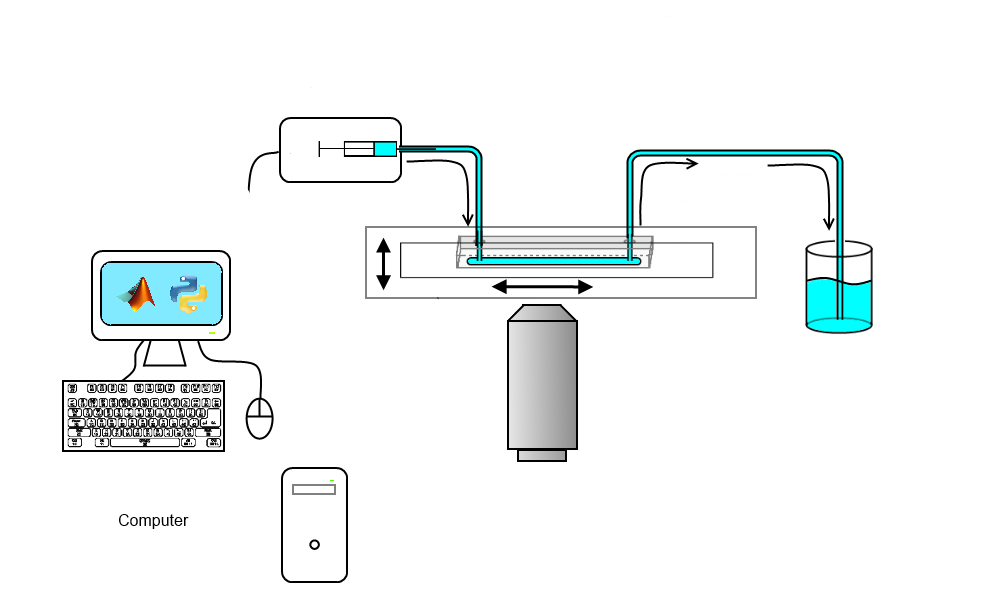
\includegraphics[width=0.8\textwidth]{figures/method/setupsketch.png}
\caption{Sketch of the set up. The computer-controlled stage moves over the microscope. The pump reverses when the tracked particle gets close to the inlets of the channel. A CCD camera connected to the microscope records the dynamics of the particle as movies. Not pictured is the optical tweezer constructed by Laas~\cite{alexanderThesis} used to control the initial conditions of the particle between measurements.	\label{fig:setupsketch}}
\end{figure}

% Have both this zoomed out and the zoomed in view I think
\begin{figure}[H]
\centering
\includegraphics[width=0.8\textwidth]{figures/method/ExperimentalOverview.jpg}
\caption{Overview of the set up. The microscope to the left and the syringe pump to the right. In the center is the channel and the outlet container is seen behind it. The CCD camera is mounted on the left side of the microscope and cannot be seen in this picture.}\label{fig:setuppicture}
\end{figure}


The microfluidic channel is \unit[40]{mm} long, \unit[2.5]{mm} wide and approximately \unit[150]{$\mu$m} deep. The channel is made from Polydimethylsiloxane (PDMS) and plasma bonded to a microscope slide. A more detailed description of the process can be found from the Center for Computer Integrated Systems for Microscopy and Manipulation~\cite{PDMS}. This material and procedure is chosen so that a channel that gets filled with dirt or breaks can cheaply and easily be replaced. Dirt in this case refers primarily to bubbles and to particles that stick to the glass or the PDMS. PDMS is non-reactive which means surface effects and other interactions with the particles are not a concern. PDMS is also highly transparent which means the light from the microscope illuminator won't be blocked or distorted before hitting the particles. A sketch of the channel can be seen in Figure \ref{fig:channelsketch}, and a photograph of an actual channel in Figure \ref{fig:channelpicture}.

\begin{figure}[H]
\centering
\begin{subfigure}[b]{0.45\textwidth}
\includegraphics[width=0.9\textwidth]{figures/method/channelDetail.pdf}
\caption{Sketch of the channel}\label{fig:channelsketch}
\end{subfigure}
\begin{subfigure}[b]{0.45\textwidth}
\includegraphics[width=0.9\textwidth]{figures/method/ChannelZoomed.jpg}
\caption{Picture of the channel}\label{fig:channelpicture}
\end{subfigure}
\caption{A sketch of the channel as well as a picture of the channel as it is set up during a measurement. The channel is only \unit[150]{$\mu$m} deep, but the PDMS surrounding it is around 15 mm to try and prevent the channel from expanding and contracting too much.}
\label{fig:channel}
\end{figure}

% rewrite
In order to find the maximum flow speed of the channel, we need to know the flow profile. Using the software employed by Johansson \cite{AntonThesis} which in turn is using results from Zheng~\cite{flowprofile}, we solve the Poisson equation in a rectangular channel to obtain the flow profile. The solution for our channel measurements can be seen in Figure \ref{fig:flowprofile}. 
Integrating the flow profile over the entire surface gives an effective flow area, essentially how large the channel 'actually' is. 
Using the flow profile from Figure \ref{fig:flowprofile} we find that the effective flow area is $\unit[0.14]{mm^2}$. With a pump rate of \unit[7.5]{$\mu$l/minute} we get a maximum speed of $v_{max} =$\unit[0.90]{mm/s} for the liquid.

% PIcture of the channel meassurements here 


% Picture of channel flow profile
\begin{figure}[H]
\begin{center}
\includegraphics[width=0.7\textwidth]{figures/method/flowprofile.pdf}
\end{center}
\caption{The theoretical estimation of the flow profile. Image generated with software from Johansson \cite{AntonThesis}, used with permission.}
\label{fig:flowprofile}
\end{figure}

\noindent We need to confirm that the flow is Stokes' flow and thus has no inertial effects. We can calculate the maximum Reynolds number using eq \ref{eq:reynolds}. Using the \unit[3]{$\mu$m} length of the particles as our characteristic length, and our maximum flow speed $v_{max}$:

\begin{equation}
\operatorname{Re} = \frac{U W \rho}{\mu} 
\leq \frac{9.0\cdot 10^{-4} \cdot 3 \cdot 10^{-3} 2.5 }{24 \cdot 10^{-3}} 
\approx	 2.78  \cdot 10^{-6} \ll 1.
\end{equation}

\noindent This satisfies the conditions of validity for the Jeffery equations. 



\subsection{List of equipment}
 The equipment used during the experiment is as follows
\begin{itemize}
\item Leica DFC350 FX digital camera 
\item Nikon Eclipse TE 300 microscope
\item Nikon 60x water immersion objective
\item Märzhäuser Wetzlar 'LStep-eco' step engine
\item CMA 4004 syringe pump
\item Ytterbium fiber laser  % What laser?
\end{itemize}

%
%\subsection{Density matching}
%\begin{equation}
%\rho_{a} = 	\frac {m_{a}}{V_{a}} =
%				\frac{V_{b}\rho_{b} + V_{mix}\rho_{mix}}{V_b + V_{mix}} 
%\end{equation}
%So if we want to find $V_{mix}$ we get
%\begin{equation}
%V_{mix} = \frac{ V_{b}(\rho_{b} - \rho_{a})}{\rho_{a} - \rho_{mix}} 
%\end{equation}
%
	
\section{Problems and improvements}
As previously mentioned this thesis is a continuation of work done by Mehlig \emph{et al}, Einarsson \emph{et al} and Mishra \emph{et al} \cite{AntonThesis, JonasExperiment, Mishra}. Their results were promising but there were a number of key limitations and problems that need to be solved in order to improve the results. They can be summarized as:
\begin{enumerate} \label{list:problems}
	\item The particles 
	\begin{itemize}
		\item Very few particles used in previous experiments were sufficiently symmetric to have quasi periodic orbits. Most were visibly bent or uneven, see figure \ref{fig:oldparticles}
		\item The average aspect ratio of the particles was very high which meant there were very few flips along a stretch.
		\item The width of the particles could not be measured, is not uniform and very small which makes estimates of the aspect ratio hard.
		\item The particles could not be trapped with an optical tweezers due to low transmittance.
	\end{itemize}
	\item The PDMS in the channel was very jagged which caused a great deal 
			of noise unless the focus was in a very narrow band.
	\item Manual tracking of particles was time consuming and mentally draining.
	\item Bubbles are difficult to avoid when setting up the experiment
\end{enumerate}


\subsection{Particles and channel}
\label{sec:particle_improves}
\begin{figure}[H]
\centering
\begin{subfigure}[b]{0.45\textwidth}
\includegraphics[width=0.9\textwidth]{figures/improvements/oldparticle2.png}
\caption{Particle 13 from July 2012}
\end{subfigure}
\begin{subfigure}[b]{0.45\textwidth}
\includegraphics[width=0.9\textwidth]{figures/improvements/oldparticle3.png}
\caption{Particle 22 from July 2012}
\end{subfigure}
\caption{Two typical particles from the previous setup. Note that these particles are selected for being among the most symmetric in the sample and yet they are noticeably bent.}
\label{fig:oldparticles}
\end{figure}



In order to solve the issues with the polymer particles, they were replaced with glass particles from Nippon Glass, Japan \cite{Particles}. 

These new particles are made from LCD spacing rods that are broken into pieces. This means that they are essentially broken cylinders with very homogeneous widths but some variation in length. Two different batches of particles were used, one with a $3\mu m$ diameter and one batch with $5 \mu m$ diameter. All the measurements presented in this thesis are using the $3 \mu m$ width particles. This is primarily as they were more easily controlled with the optical tweezers and because they sink or float more slowly. 

The symmetries of the particles were investigated with help from Stefan Gustafsson by taking images with an 
ESEM (Environmental Scanning Electron Microscope) shown in Figure \ref{fig:particlepictures}. We see that the 
particles are uniformly smooth along the sides but have varyingly jagged edges causing different degrees of asymmetry. 

Figure \ref{fig:roundparticle} shows a particle along the main axis. We see that it is a circular shape
with no discernible deformation or asymmetry whereas Figure \ref{fig:particlepictures} shows the jagged edges of several particles. 


\begin{figure}[H]
\centering
\begin{subfigure}[3a]{0.40\textwidth}
\includegraphics[width=\textwidth]{figures/method/semizoomed.png}
\caption{A detailed view \\ of a number of particles.}
\end{subfigure}\hspace{1em}%
\begin{subfigure}[3b]{0.40\textwidth}
\includegraphics[width=\textwidth]{figures/method/zoomedbroken.png}
\caption{The jagged edge of a particle \\ in detail.}
\end{subfigure}
\caption{Pictures of the glass particles that were used. Their width is uniform and there is a noticeable variation in asymmetry. Some particles show very clearly jagged edges while other appear very smooth. This suggests that they should have quite different $\epsilon$ and then exhibit quite different behaviour. Obtained with the help of Stefan Gustafsson}
\label{fig:particlepictures}
\end{figure}
 
\begin{figure}[H]
\centering
\begin{subfigure}[3a]{0.40\textwidth}
\includegraphics[width=\textwidth]{figures/method/symmetric.png}
\caption{What appears to be a highly \\ symmetric particle.}\label{fig:symmetricparticle}
\end{subfigure}\hspace{1em}%
\begin{subfigure}[3b]{0.40\textwidth}
\includegraphics[width=\textwidth]{figures/method/round.png}
\caption{A top down view of a particle.}\label{fig:roundparticle}
\end{subfigure}
\caption{Pictures highlighting the roundness of the particles as well as the apparent symmetry of some particles. Obtained with the help of Stefan Gustafsson}
\label{fig:particlepictures2}
\end{figure}

\noindent Figure \ref{fig:roundparticle} and \ref{fig:symmetricparticle} are the same as can be seen in Laas~\cite{alexanderThesis} Figure 5.2(c) and 5.2(b) respectively. 

The particles satisfy the symmetry conditions but are made of glass with a density of approximately 
\unit[2.57]{g/cm$^3$} at \unit[20]{C$^\circ$}. This is significantly higher than that of water with a density of 
\unit[1]{g/cm$^3$} at \unit[20]{C$^\circ$} and glycerol with a density of \unit[1.5]{g/cm$^3$}. In order to keep the particles buoyant the water soluble Sodium metatungstate is added to the liquid. Sodium metatungstate dissolved in water has a density of \unit[2.94]{g/cm$^3$} at \unit[20]{C$^\circ$} when fully saturated. To increase the viscosity of the liquid around 8\% glycerol is added and the liquid was measured using a MCR 302 rheometer to have a dynamic viscosity of \unit[$24\cdot 10^{-3}$]{Pa s}.

The problem with using these cylindrical particles is that the asymmetric cylinders with jagged edges do not have the same symmetries as the triaxial particles. The triaxial particles with distinct $a_2$ and $a_3$ have $2$-fold rotational symmetry around every axis whereas this is not true for the cylinders. We do not know how this symmetry difference effects the equations of motion and in consequence the orbits, Poincaré maps, and winding numbers. We assume that we can approximate a jagged cylinder with a triaxial particle: Further theoretical development will prove if this is correct or not.


A problem in finding and tracking a particle was that the surface of the PDMS was very uneven and sharp ridges along the length of the channel appear as in figure \ref{fig:unpolished} unless the focus was in a relatively narrow depth of the channel. 
 
 \begin{figure}[H]
 \centering
 \begin{subfigure}[3a]{0.40\textwidth}
 \includegraphics[width=\textwidth]{figures/improvements/unpolished.png}
 \caption{An unusually severe case of the PDMS edges creating noise.}\label{fig:unpolished}
 \end{subfigure}\hspace{1em}%
 \begin{subfigure}[3b]{0.40\textwidth}
 \includegraphics[width=\textwidth]{figures/improvements/polished.png}
 \caption{After being polished there is no trace of such ridges.}\label{fig:polished}
 \end{subfigure}
 \caption{Pictures highlighting the roundness of the particles as well as the apparent symmetry of some particles. It should be noted that although there are no apparent rough edges there was no way to rotate a sample so there might very well be asymmetries on the side of the particle that we cannot see.}
 \label{fig:polisheffect}
 \end{figure}
 

This was fixed by polishing the copper mold in which the PDMS channels are formed with a silicate abbrasive (Autosol) and emery cloth. This was shown to remove all visible scratches from the mold and thus from the PDMS. As seen in Figure \ref{fig:polished} no scratches can be detected.

\section{Automated tracking}
%GENERAL LAYOUT
%
%Why we want tracking 
%
%The differences between tracking and tracking
%
%The methods used
%
%The limitations
%
%1) Why we want tracking

One of the most time consuming aspects of making measurements is manually tracking a particle using the movable stage as described in section \ref{sec:exp_setup}. Depending on the flow rate and the number of stretches and measurements desired for a particle it can take up to several hours. Thus one of the primary targets for improvement as discussed by Johansson \cite{AntonThesis} was automate the camera tracking. This would speed up measurements and allow for a larger data set to be gathered. 

Such a tracking was implemented using Python and the external packages \texttt{OPENCV}, \texttt{NumPy}, \texttt{SciPy}, \texttt{ImageMagick} and \texttt{ctypes}. The goal of the tracking is relatively similar to the tracking described in \ref{sec:particleidentification} and more in detail in Johansson \cite{AntonThesis}. The main difference is that the tracking describe in this section moves the actual stage and control the pump in real time whereas Johansson tracking tracks the particle in the movie after manual measurements have been made. This produces some different problems which are detailed below. 

\subsection{Acquiring the image}
The first step in tracking a particle is to acquire the image from the microscope in order to identify (and track) the particle. However the Leica DFC350 FX camera only works with the proprietary Leica software which means there is no easy way to get the image straight from the camera in real time. To solve this we use the \texttt{ImageGrabber} package in \texttt{Python} to isolate the camera image from the screen by cropping the image aquired. While being a very short program it still takes ca \unit[50]{ms} per frame. Each frame is stored as a matrix $\mathbf{F}$ with brightness values ranging from 0 to 255.

\subsection{Reducing noise}
In order to reduce noise from the image we first reduce the static noise caused by dirt, scratches and other defects in the microscope and on the camera lens, as shown in figure \ref{fig:origFrame}. As the noise is static it is the only thing that will remains if we compute an average image $\bar{\mathbf{F}}$. After taking $N$ images and denote them $\left\{\mathbf{F}_1,\mathbf{F}_2 ... \mathbf{F}_N \right\}$ the average images $\bar{\mathbf{F}}$ is given by 

\begin{equation}\label{eq:averageFrame}
\bar{\mathbf{F}} = \frac{1}{N}\sum\limits_{i=1}^{N} \mathbf{F}_i.
\end{equation}

An example of such an average image can be seen in figure \ref{fig:averageFrame}. The static noise is then removed from each frame using eq 3.1 from Johansson \cite{AntonThesis}.

\begin{equation}
\widetilde{\mathbf{F}_{i}} = \mathbf{F}_i - \bar{\mathbf{F}} + (F_i^*\mathbf{I})
\end{equation}

\noindent where $\F_i^*$ is the average brightness of the frame $\mathbf{F}_i$, $\widetilde{\mathbf{F}_{i}}$ is the corrected frame and $\mathbf{I}$ is a matrix of ones. The result can be seen in figure \ref{fig:fixedFrame}. 




\subsection{Contour detection and selection}
The edges of the captured image are detecting using the Canny edge detector from the OpenCV package. The canny edge detector takes two thresholds for finding edges, $\tau_1$ and $\tau_2$ with $\tau_1 > \tau_2$. $\tau_1$ is used for finding initial edges and $\tau_2$ is used on pixels adjacent to ones already found. For more details on how the Canny Edge detector works see the original paper by Canny from 1986\cite{Canny}. Once an edge image has been generated, we use the OpenCV command, \texttt{Contours} which returns a list of every contiguous group of edge pixels.  We denote these contours $\left\{C_1, C_2 \ldots C_M \right\}$ and each contour contains $M^c_i$ pixels, $C_i = \left\{p^i_1, p^i_2 \ldots p^i_{M^c_i}\right\} $. If the image is not too noisy and we have chosen the threshold values to the edge detection correctly, this should include the particle as a contour. 

In order to identify the particle contour  a few techniques are used. First, contours whose total size $ M_c^i$ is less than some minimum value, $ n_{min}$ or larger than some maximum value $n_{max}$ are ignored. Then the average position $\mathbf{P}_i$ of each contour $C_i$ is calculated as the average pixel position

\[
\mathbf{P}_i = \sum_{j=1}^n p_j/n
\]

which is used to find the distance $D_i$ between each position $\mathbf{P}_i$ and the expected position $\mathbf{E}$. The expected position is first frame the center of the image and thereafter we assumed the particle have assumed to have constant velocity. So we have 

\[
D_i = \left|\mathbf{P}_i - \mathbf{E}\right|
\]

Finally a 'thinness value' for each contour $\zeta_i$ is calculated using

\begin{equation}\label{eq:thinness}
\zeta_i =  \left(\frac{d_{i, max}^2}{M_c^i}\right)^2,
\end{equation}. 

where $d_{i,max}$ is the longest distance between two pixels in the contour $C_i$.

Finally a weighted score $S_i$ is assigned to each contour based on its position and thinness using

\begin{equation}
S_i = w_{thin}\zeta_i + \frac{w_{pos}}{D_i}
\end{equation}
\noindent where $w_{thin}$ is a weighting constant for the thinness and $w_{pos}$ is a weighting constant for the position. The contour with the highest score is chosen unless it is lower than some worst acceptable score $S_{min}$

\subsection{Adjusting the camera velocity}
After two detections of the particle $\mathbf{P}(t_0)$ and $\mathbf{P}(t_1)$, there will have been some change in position which we will refer to as the relative velocity $\mathbf{v}_{rel}$ and the velocity of the step engine as $v_{step}$ and the correctional change in velocity of the step engine $\mathbf{v}_{corr}$.

If the velocity is larger than some threshold $v_{thresh}$ the step engine velocity is changed by
\[
\mathbf{v}_{corr} = \mathbf{v}_{rel}\zeta
\]
where $\zeta < 1$ is damping to prevent too sudden changes. If the position of the particle is too far from the center of the image the velocity of the step engine is changed by .
\[|
\mathbf{v}_{corr} = \frac{\mathbf{P}(t_1)}{\left|\mathbf{P}(t_1)\right|}v_{\epsilon}
\] 
where $v_{\epsilon}$ is a small incremental velocity.


\subsection{Time Considerations}\label{sec:time considerations}
A higher frame rate will allow for greater predictive power and increase stability as the error between frames is 
reduced. Reducing computational time of each task is important for optimizing the tracking, which also means knowing 
what tasks are the most demanding. A list of the different tasks and their average execution times can be seen in table 
\ref{tab:benchmarks}


\begin{table}[H]
 \begin{tabular}{l | c | c } 
 Task  			&  Average time & Std deviation \\
 Capture screen & 41 			& 14 \\
 Find edges 	& 78			& 23 \\
 Change velocity& 230			& 62 \\
 \end{tabular}
 \caption{}
 \label{tab:benchmarks}
\end{table}

We see that the FPS is limited primarily by three routines: The screen capture routine, the change velocity routine and finally the save position routine. The first and last are unavoidable and must be done every frame by definition if we are interested in knowing the particles position as well as possible. This means we simply want to use the velocity correction as little as possible. Since the time constraint is in the communication with the step engine, there is not any optimization to be done here, at least not within the scope is this thesis. 
     

\section{Summary of improvements}
To conclude we return to the problems listed in in section \ref{list:problems} 

\begin{enumerate} \label{list:solutions}
	\item The particles are now all symmetric to be used for measurements
	\item The particles have low aspect ratios and uniform widths allowing which makes accurate estimations of size possible
	\item The lower aspect ratios means there are more flips that can be used to estimate the orbit.
	\item Particles are made from glass meaning they can be trapped using optical tweezers.
	\item The PDMS in the channel is now smooth enough to not be noticed with the microscope.
	\item Manual tracking is still necessary when tracking with the optical tweezers.
	\item Bubbles are still an issue, but are reduced as one gets more experienced in setting up the experiment.
\end{enumerate}

 Part 2: Measurements and Analysis


\part{Data analysis and results}
\chapter{Data analysis}
Once a movie had been recorded we want to estimate the dynamics of the particle. This is done in several steps. 

\subsection{Particle identification}

The first step is to reduce the static noise from the movie caused by dirt, scratches and other defects in the microscope and on the camera lens as can be seen in figure \ref{fig:origFrame}As the noise is static and everything else changes this is a simple matter of computing an average frame

\begin{equation}\label{eq:averageFrame}
\bar{F} = \frac{\sum\limits_{n=1}^{N} F }{den}
\end{equation}

an example of such an average frame can be seen in figure \ref{fig:averageFrame}. This is then removed from the camera frame and the result can be seen in figure \ref{fig:fixedFrame}. After this we apply a smoothing function and Canny edge detection \cite{Canny} and then fill the resulting edge. The resulting pixels are then fit to an ellipse as described in \cite{AntonThesis, EllipseFit}. The filled contour and the fit ellipse can be seen in figure \ref{fig:edgeFrame}.

\begin{figure}[H]
\centering
\begin{subfigure}[3a]{0.40\textwidth}
\includegraphics[width=\textwidth]{figures/method/static1.png}
\caption{A typical raw video frame.}\label{fig:origFrame}
\end{subfigure}\hspace{1em}%
\begin{subfigure}[3b]{0.40\textwidth}
\includegraphics[width=\textwidth]{figures/method/static3.png}
\caption{The average frame $\hat{F}$ from eq \ref{eq:averageFrame}.}\label{fig:averageFrame}
\end{subfigure} \\

\begin{subfigure}[3a]{0.4\textwidth}
\includegraphics[width=\textwidth]{figures/method/static2.png}
\caption{The same frame after noise reduction}\label{fig:fixedFrame}
\end{subfigure}\hspace{1em}%
\begin{subfigure}[3a]{0.4\textwidth}
\includegraphics[width=\textwidth]{figures/method/edge.png}
\caption{After edge detection and ellipse fitting}\label{fig:edgeFrame}
\end{subfigure}

\caption{These pictures show a simplified version of the image analysis from raw image to estimated particle position}
\label{fig:detection}
\end{figure}

\subsection{Estimation of orientation}

The ellipsoid we get is then our best approximation of the projection of the actual particle. In order to normalize $\mathbf{n}$ we need to know the length of the particle. However as it was shown by Leal that the particle will always spend a majority of its time aligned with the flow, ie aligned with the camera which means that by simply calculating the length $L$ every frame and finding the mode of the distribution we will find a good estimate of L. 

So given an ellipsoid with length $l_e$, width $d_e$ and angle $\phi_p$ we find 

\begin{align} \label{eq:project}
p_x  &= l_e*sin(\phi_p) \\
p_z  &= l_e*cos(\psi_p) 
\end{align}

with x and z projection $p_x$ and $p_z$ we can get $n_x$and $n_z$ as well as $n_y$via 
\begin{subequations}\label{eq:normalize}
\begin{align}
n_x 	&= \frac{p_x}{L} \\
n_z 	&= \frac{p_z}{L} \\
n_y		&= \sqrt{1 - n_x^2 - n_z^2}
\end{align}
\end{subequations}


\subsection{Width compensation}\label{sec:width_compensation}
Up until this point we have assumed that the particle is a \emph{thin} rod so that the projection $\mathbf{p}$ onto the x and z-axes give us an accurate estimate of $\mathbf{n}$. However when we are projecting 'thick' partcle with length L and width D we get $\mathbf{n}'$. At $\phi = 0$ this is

\begin{equation}
\mathbf{n}' = n_z' = n_z\cos(\theta)  + D\sin(\theta) 
\end{equation}

which is illustrated in figure \ref{fig:lengtherror}. 

In order to compensate for this error we modify our projection equation \ref{eq:project} to

\begin{align}\label{eq:widthCompensation}
p_x  &= (l_e - w_e)*sin(\phi_p) \\
p_z  &= (l_e - w_e)*cos(\psi_p) 
\end{align}

This will reduce the particles estimated length by $w_e$
\begin{figure}[H]
\centering
\includegraphics[width=0.6\textwidth]{figures/method/LengthError.pdf}
\caption{}\label{fig:lengtherror}
\end{figure} 



\section{Removing tracking errors}
\label{sec:brushing}
The tracking typically contain a few frames where either the view of the particle is visually obstructed or is not detected correctly 
leading to spikes in the data. To make further theoretical analysis possible the data is corrected by removing such points manually. The basis for removal is a large discontinuity in the data, and could largely be eliminated with algorithmic means. However in particular for $n_z$ it is very difficult to write an algorithm that will catch all possible edge cases. For example $n_z$ have peaks that make its derivative non continuous which means that cannot be use as a criterion. It's thus simpler to look at the analysis program and remove the points where the particle cannot be traced accurately due to noise. 

An example of data before and after correction can be seen in figure \ref{fig:brushed} and all uncorrected data files will be available at \url{http://goo.gl/jgzSXe}.

\begin{figure}[H]
\centering
\begin{subfigure}[3a]{0.40\textwidth}
\includegraphics[width=\textwidth]{figures/method/Brushing1.png}
\caption{$n_x$ time series before correction.}\label{fig:prebrush}
\end{subfigure}\hspace{1em}%
\begin{subfigure}[3b]{0.40\textwidth}
\includegraphics[width=\textwidth]{figures/method/Brushing2.png}
\caption{$n_x$ time series after correction.}\label{fig:postbrush}
\end{subfigure} \\
\caption{Shows a time series of $n_x$ before and after removing points where a significant amount of noise disturbed the tracking. } \label{fig:brushed}
\end{figure}


\section{Estimating the winding numbers}
\label{sec:windingEstimation}
As discussed in section \ref{sec:winding}, estimating the winding number for different types of orbit for one particle 
should allow for a rather accurate estimation of $\epsilon$. So in order estimate the winding number for a measured 
particle we must identify where the $\theta_1$ maxima and minima from figure \ref{fig:windingDef} occur. First, the 
$\theta_2$ maxima is located by where $n_x = 0$. A plot of such 
points can be seen in figure \ref{fig:nzNx0} where we match each $n_z$ peak with an index $i$. Unfortunately data is 
too noisy to allow for simple algorithmic approaches 
to finding good local maxima. Instead we select a number of maxima $M_1, M_2 ... M_p$ with peak index $I^M_1, I^M_2, 
..., I^M_p$  and minima $m_1, m_2, ..., m_q$ with peak index $I^m_1, I^m_2, ..., I^m_q$.

\begin{figure}
\centering
\includegraphics[width=0.7\textwidth]{figures/method/nzNx0.pdf}
\caption{The stars are plotted at the same distances in the $n_x$ and $n_z$ plots. This shows that zeros of $n_x$ and maxes of $n_z$ occur almost exactly at the same points.}
\label{fig:nzNx0}
\end{figure}

We can estimate the winding number $\hat{w}$ as the average distance between the peak indices for the maxima and minima 
i.e. 

\begin{align}
\overline{d_M} &= \frac{1}{p-1} \sum\limits_{j=1}^{p} I^M_{j+1} - I^M_{j} \\
\overline{d_m} &= \frac{1}{q-1} \sum\limits_{j=1}^{q} I^m_{j+1}- I^m_{j}\\
\hat{w}   &= \frac{\overline{d_M} + \overline{d_m}}{2}.
\label{eq:winding2}
\end{align}


In the case that we only have 1 maxima and minima we use instead that the distance between maxima and minima should be 
half a period, i.e.

\begin{equation}
\hat{w} = \left| I^M_1 - I^m_1 \right| \cdot 2
\end{equation}

\section{Matching data to theoretical orbits}
\label{sec:matchorbit}
To verify that the theoretical Jeffery orbits from \ref{sec:jeffery} are present we want to match the measurements to theoretical orbits.

To find the best matching orbit from a Poincaré map for a measurement we again utilize $P_z$, the points where $n_z$ peaks and $n_x=0$. We denote the length o f$\mathbf{P_z}$ as $N$. We are concerned with matching them with the peaks from theoretical orbits.

%To find the best matching theoretical orbit we calculate the least square distance of $\mathbf{P_z}$ against the theoretical peaks for $\epsilon \in [0.01, 0.02, ..., 0.1]$ and for $\cos(\theta) \in [-1,1]$ 
%and for $\psi \in [-\frac{pi}{2},\frac{pi}{2}]$. 

To find the best matching theoretical orbit for a measurement we compute the least square between $P_z$ and all orbits on all phase maps with $\epsilon \in [0.01, 0.02, ..., 0.1]$ for 200 consecutive different initial $\psi$ (the $x$-axis on the Poincare map). If we for each orbit denote the theoretical series of $n_z$ peaks as $\mathbf{Q_z}(\theta, \epsilon)$. We let $\mathbf{Q_z}(\theta, \epsilon)$ be of length $M > 2N$ and define $\mathbf{Q_z}(\theta, \epsilon, i)$ to be the $n_z$ series $\mathbf{Q_z}(\theta, \epsilon)$ starting at index $i$. We assign a score function $S(\theta, \epsilon, i)$ as

\begin{equation}
S(\mathbf{P}, \theta, \epsilon, i) = \frac{1}{N}\left| \mathbf{P_z} - \mathbf{Q_z}^{(i)}(\theta, \epsilon) \right|^2.
\end{equation}

\noindent An example experimental $P_z$ series matched to theoretical data is seen in Figure \ref{fig:particleB2match}.

\begin{figure}[H]
\centering
\includegraphics[width=0.7\textwidth]{figures/results/particleB/October_1_Particle_4_run_4match.pdf}
\caption{The upper figure shows the experimental $n_z$ peaks $\mathbf{P_z}$ versus the theoretical $Q_z$ for the best matching orbit. The lower plot shows where what section of the theoretical time series was used for matching, ie what $i$ from section \ref{sec:matchorbit} was chosen.}
\label{fig:particleB2match}
\end{figure}



\noindent As $\epsilon$ will not actually change for a single particle over $r$ different measurements $P_z^{(1)}, P_z^{(2)}, ..., P_z^{(r)}$, however the initial conditions $\theta$ and $i$ (the phase) will. So for each $\epsilon$ we find the best $\theta$ and $i$ using $\hat{S}(\mathbf{P}_j, \epsilon)$ 
\begin{equation}
\hat{S}(\mathbf{P}_j, \epsilon) =  \min(S(\mathbf{P}_j, \theta, \epsilon, i))
\end{equation}

\noindent and  then find the best $\epsilon$ using

\begin{eqnarray}
\epsilon_{best} = \min(\sum\limits_{j=1}^{r} \hat{S}(\mathbf{P}_j, \epsilon)^2).
\end{eqnarray}


It is important to note that this matching has a theoretical limitation. The asymmetry of our cylindrical particles is different from the asymmetry in the triaxial particles used in the theoretical models. The triaxial particles still have a rotational symetry for rotations of $\pi$ around any of the major/minor axes. This is not the case with the asymmetric cylindrical particles, which have no rotational symmetry. We therefore have to make the assumption that the difference between these two types of asymmetry is not significant and further theoretical work might reject this assumption.

% Refer to some matched plots once I have added those. I THINK basically everythig should already be in the saved plots and data folder. 


\chapter{Results}
During the work of this thesis around 300 movies of particles have been recorded with gradual improvements to the setup in terms of density matching, particle density, bubble elimination etc. In this section we will present the data from three movies of two different particles. One referred to as particle A, the other as particle B. The measurements in this section was done together with Alexander Laas.

Each measurement was started at an approximate depth $D$ and at position $p_0 = (x_0, z_0)$ in the channel relative to the inlet on the right, closer to the pump. Since we want the shear to be entire in the $y$ direction we would want to be as close to $z_0 = 0$ as possible, but variations less than \unit[1]{mm} should still have virtually identical shear.

In the time series plots below such as figure \ref{fig:particleA1}, the circular and star markers indicate the peaks used for estimating the winding number as explained in section \ref{sec:windingEstimation}. A circle is an estimated minima $m_i$, stars an estimated maxima $M_i$.

\newpage
\section{Measurements}
\subsection{Measurements of particle A}
Particle A was measured on October 11 in 2013. Two of the measurements retraced their orbits very well: measurement 1 and measurement 2 which can be seen in Figure \ref{fig:particleA1} and Figure \ref{fig:particleA2} respectively. Measurement 1 was started with initial condition $n_z \approx 0$ and showed quasi periodic behaviour with a periodic change in amplitude for $n_z$ peaks. Measurement 2 was started with initial condition $n_z \approx 1$ and showed periodic behaviour with very constant $n_z$ peaks. 

Other measurement had reversals where the orbit changed considerably, two examples are seen in Figure \ref{fig:particleA3} and \ref{fig:particleA4}. All measurement data for particle A can be found at \url{goo.gl/jgzSXe} where particle A is referred to as particle 2 from October 11. 


\subsubsection{Measurement 1}
\begin{figure}[H]
\begin{center}
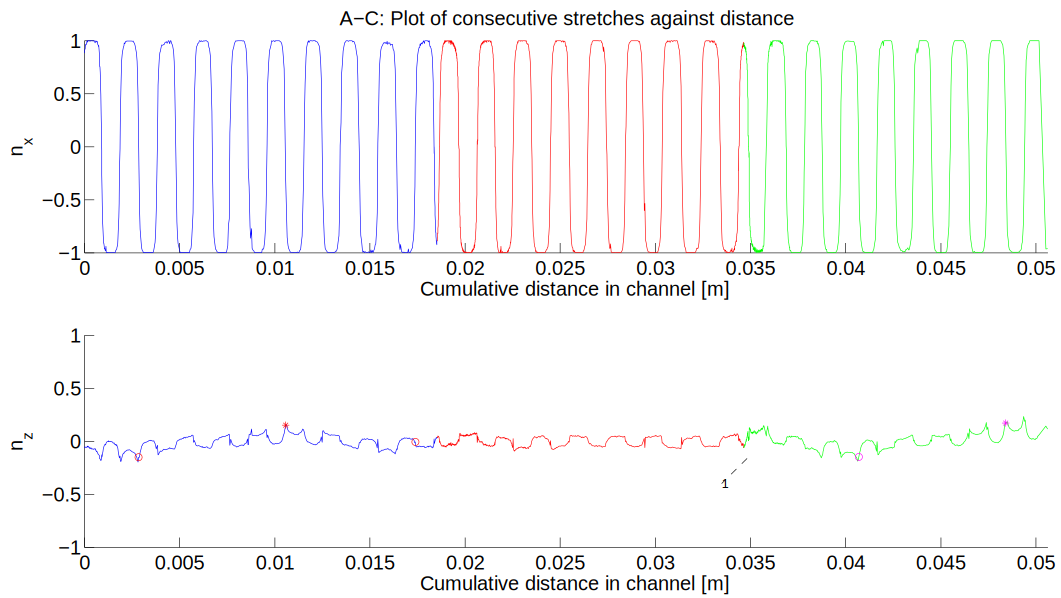
\includegraphics[width=0.7\textwidth]{figures/results/particleA/October_11_Particle_2_run_2_winding.pdf}
\end{center}
\caption{The $n_x$ and $n_z$ components of the particle for measurement 1 against cumulative distance in channel. Despite being very close to a centre orbit there is limited quasi-periodic behaviour as the peaks stay close to 0. The very flattened peaks compared to a low $n_z$ orbit in \ref{fig:orbitparams} are a result of the width compensation discussed in section \ref{sec:width_compensation}. This particle started $x_0 = 9.8 mm, z_0 = 8.9924 \mu m$ and $D \approx 90\mu$m. This is the same measurement as is used in Figure 6.20 in Laas thesis~\cite{alexanderThesis}}
\label{fig:particleA1}
\end{figure}


\subsubsection{Measurement 2}
\begin{figure}[H]
\begin{center}
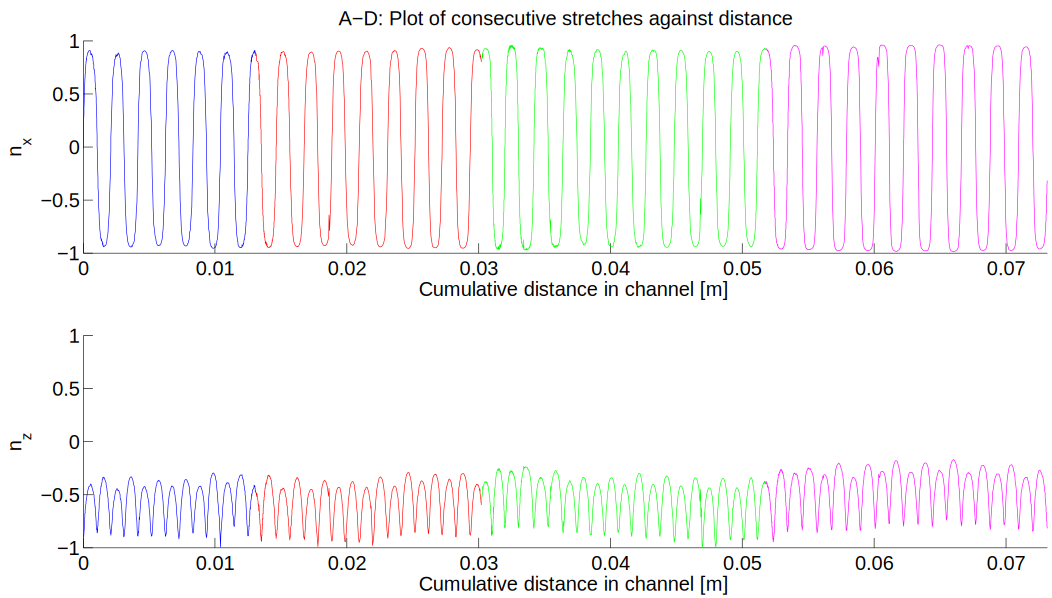
\includegraphics[width=0.7\textwidth]{figures/results/particleA/October_11_Particle_2_run_3_A.pdf}
\end{center}
\caption{The $n_z$ and $n_x$ components for measurement 2 against cumulative distance. The $n_z$ component is consistently close to 1 at the peaks. 
The particle started at $ x_0 = 26.0 \text{mm}, z_0 = 275\mu\text{m}, D\approx 105\mu$m. This figure is the same as Laas~\cite{alexanderThesis} Figure 6.21}
\label{fig:particleA2}
\end{figure}

\subsubsection{Measurement 3}
\begin{figure}[H]
\begin{center}
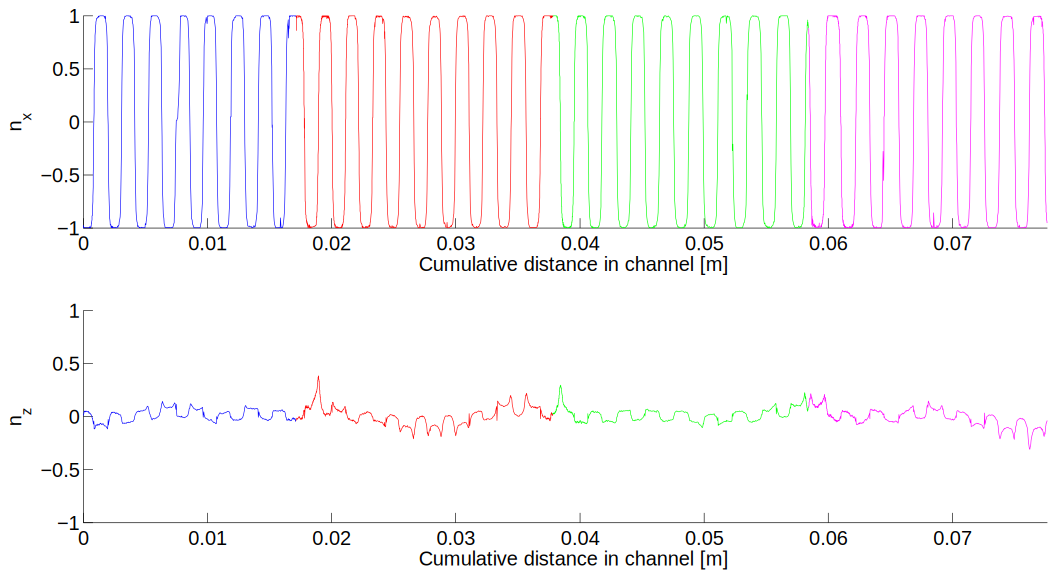
\includegraphics[width=0.7\textwidth]{figures/results/particleA/October_11_Particle_2_run_6_A.pdf}
\end{center}
\caption{The $n_z$ and $n_x$ components for measurement 3 against cumulative distance. The larger peaks that occur after the reversals are not the cause of a tracking error but can be seen clearly in the films. The reversal of the flow is started when the particle is next to the point marked (3) which is also where there is a change in $n_z$ component. The particle started at $ x_0 = 12.3 \text{mm}, z_0 = 160 \mu\text{m}, D \approx 100\mu$m.}
\label{fig:particleA3}
\end{figure}



\subsubsection{Measurement 4}
\begin{figure}[H]
\begin{center}
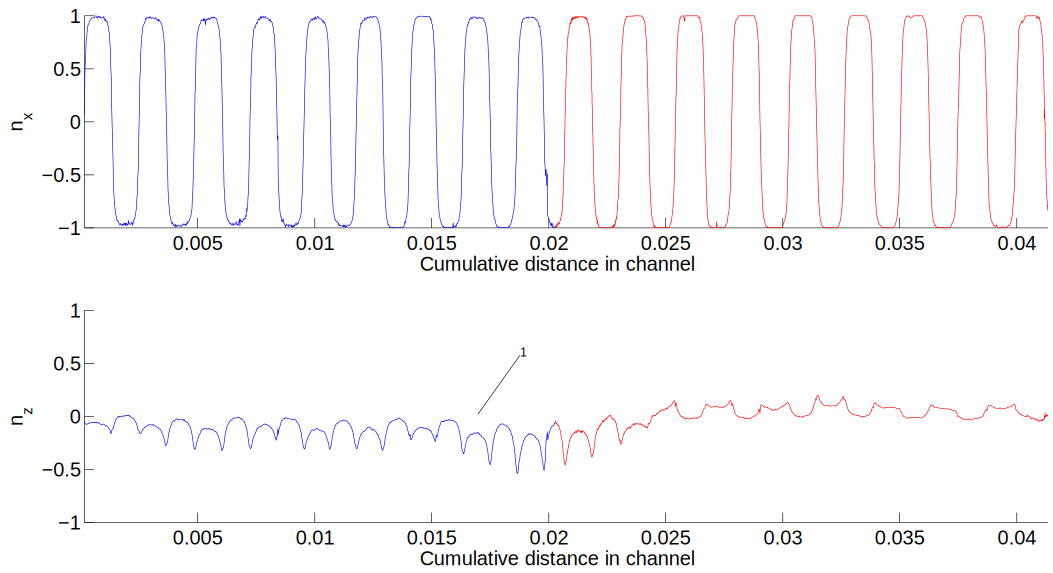
\includegraphics[width=0.8\textwidth]{figures/results/particleA/October_11_Particle_2_run_1_A.pdf}
\end{center}
\caption{The $n_z$ and $n_x$ components for measurement 4 against cumulative distance. The flow is reversed when the particle is at the point marked by (1) and we can see that the peaks around the reversal are larger than for the rest of the measurement. Started at $x_0 = 8.7 mm, z_0 = 16\mu m, D \approx 95\mu$m.}
\label{fig:particleA4}
\end{figure}

\subsubsection{Measurement 5}
\begin{figure}[H]
\centering
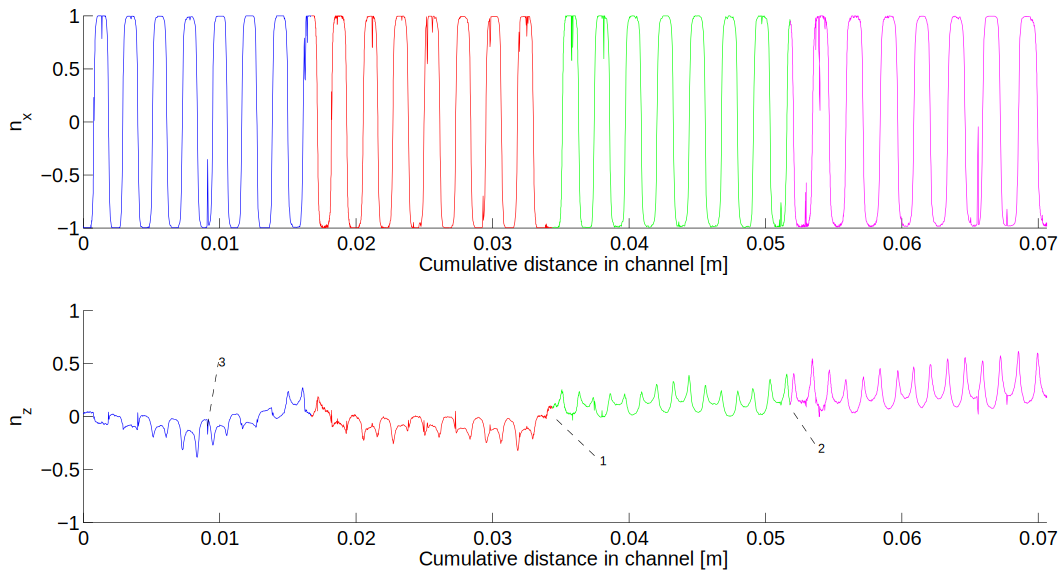
\includegraphics[width=0.8\textwidth]{figures/results/particleA/October_11_Particle_2_run_4_A.pdf}
\caption{The $n_z$ and $n_x$ components for measurement 5 against cumulative distance. At the point marked by (1) $n_z$ changes drastically at the reversal which occurs at the side of the channel closer to the pump. Although there is also some change in the orbit at the reversal marked by (2) it does not move comparably far on the S.O.S. There are a number of small peaks in the data such as the one indicated by (3) which is a consequence of insufficient removal of tracking errors, see Section \ref{sec:brushing}. The particle started at $x_0 = 10.7 mm, z_0 = 240 \mu m, D \approx 60\mu m$.}
\label{fig:particleA5}
\end{figure}

\subsection{Measurements of particle B}
Particle B was measured on October 1 2013. Particle B has four measurements for which most reversals showed little change in orbit. These are shown below in Figures \ref{fig:particleB1}, \ref{fig:particleB2}, \ref{fig:particleB3} and \ref{fig:particleB4}. There were also problematic measurements of particle B analogous to those for particle A, but they have not been included in this section for brevity. All measurement data for particle B can be found at \url{goo.gl/jgzSXe} where particle B is referred to as particle 4 from October 1. 

\subsubsection{Measurement 1}
\begin{figure}[H]
\begin{center}
\includegraphics[width=0.7\textwidth]{figures/results/particleB/October_1_Particle_4_run_2_winding.pdf}
\end{center}
\caption{The $n_z$ and $n_x$ components for measurement 1 against cumulative distance. The first two and the last two stretches the particle retraces its motion very closely during the reversals. In the reversal between these two reversals there is a large change in orbit which begins at (1) where the flow is starting to revert. This reversal occurs at the end of the channel closer to the pump. Starts at $ x_0 = 9.3$mm $,z_0 = 35\mu m, D \approx 100\mu m$. This is the same measurement as is used in Figures 6.2 and 6.4 in Laas thesis~\cite{alexanderThesis}}
\label{fig:particleB1}
\end{figure}
	


\subsubsection{Measurement 2}

\begin{figure}[H]
\begin{center}
\includegraphics[width=0.7\textwidth]{figures/results/particleB/October_1_Particle_4_run_4_A.pdf}
\end{center}
\caption{The $n_z$ and $n_x$ components for measurement 2 against cumulative distance. The orbit is mostly constant orbit with $n_z \approx 1$ at the peaks. The reversals at (1) and (3) both change the orbit slightly however the difference between the peaks is small and the best matched theoretical orbits in Figure\ref{fig:October1Particle4runs2and2Orbits} are similar before and after reversals. There is missing data at (2) and (4) where the particle was no able to be tracked. The particle started at $x_0 = 28.6$mm, $z_0 = 72\mu$m, $D = \approx 85\mu$m. This is the same measurement as is used in Figure 6.8 in Laas thesis~\cite{alexanderThesis}}
\label{fig:particleB2}
\end{figure}

\subsubsection{Measurement 3}
\begin{figure}[H]
\begin{center}
\includegraphics[width=0.7\textwidth]{figures/results/particleB/October_1_Particle_4_run_5_winding.pdf}
\end{center}
\caption{The $n_z$ and $n_x$ components for measurement 3 against cumulative distance. The initial condition is $n_z \approx 0$ and the sign changes periodically. Started at $x_0 = 2.7 mm, z_0 = 76\mu m, D \approx 90\mu$m. This is the same measurement as is used in Figures 6.10 and 6.12 in Laas thesis~\cite{alexanderThesis}}
\label{fig:particleB3}
\end{figure}


\subsubsection{Measurement 4}
\begin{figure}[H]
\begin{center}
\includegraphics[width=0.7\textwidth]{figures/results/particleB/October_1_Particle_4_run_3_winding.pdf}
\end{center}
\caption{The $n_z$ and $n_x$ components for measurement 4 against cumulative distance. While the changes are not large change in $n_z$ there is a periodic variations that could correspond to a sign preserving quasi-periodic orbit. Started at $x_0 = 12.9 mm, z_0 = 21\mu m, D \approx 85\mu$ m}
\label{fig:particleB4}
\end{figure}
\section{Diagnostic plots}

A number of diagnostic measurements were made for each particle to find possible problems with the setup. In this section we only show the diagnostic measurements from measurement 1 for particle A, and from measurement 2 for particle B but all diagnostic plots can be found at \url{http://goo.gl/jgzSXe}.


\begin{figure}[H]
\begin{center}
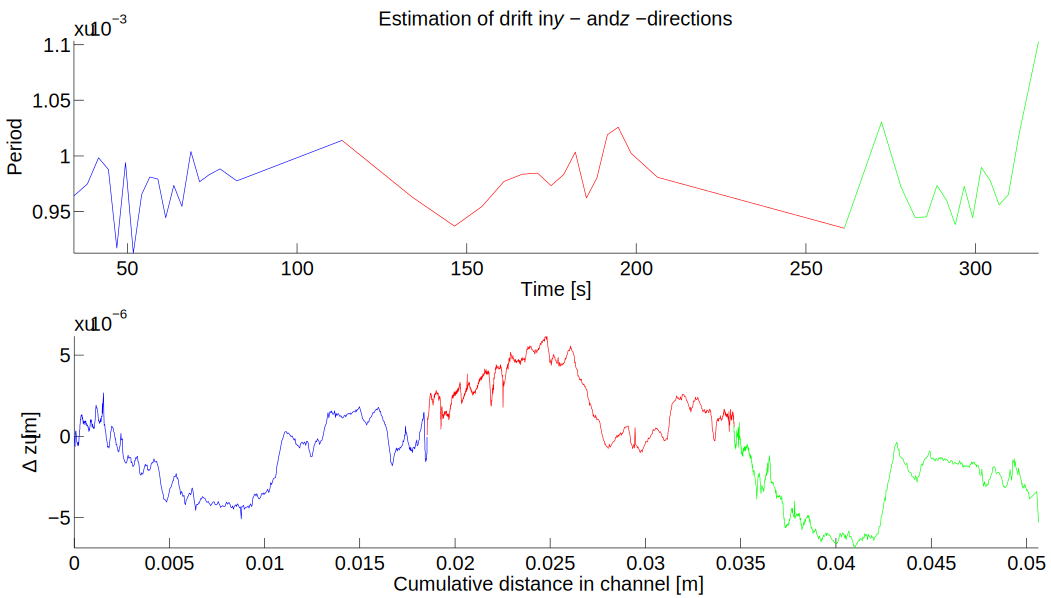
\includegraphics[width=0.7\textwidth]{figures/results/particleA/October_11_Particle_2_run_2_B.pdf}
\end{center}
\caption{The estimation of drift in $y$ and $z$ direction for Particle from measurement 1. Upper figure is the estimation of the sinking of the particle, the lower figure is the measured z position in the channel against cumulative distance. }
\label{fig:particleAsink}
\end{figure}

\begin{figure}[H]
\centering
\includegraphics[width=0.7\textwidth]{figures/results/particleB/October_1_Particle_4_run_4_B.pdf}	
\caption{The estimation of drift in $y$ and $z$ direction for Particle from measurement 1. Upper figure is the estimation of the sinking of the particle, the lower figure is the measured z position in the channel against cumulative distance.}
\label{fig:particleB2sinking}
\end{figure}



The center of mass movement in the direction perpendicular to the flow direction $x$ is seen in Figures \ref{fig:particleAsink} and \ref{fig:particleB2sinking}. Movement in the $y$ direction, i.e. sinking or floating, was measured by plotting the period of each flip against time as in the upper figure. The period here refers to the distance $\Delta_i$ between two successive zeros for $n_x$ relative to the first such distance $\Delta_0$. If there is no clear trend to higher or lower values it implies that there is little sinking or floating. 

The movement in the z coordinate is very small relative to the movements in the x direction. We can see that Z-direction movements along one stretch are on the order of $10\mu m$ compared to the x direction which is on the order of $2\cdot 10^4 \mu m$.The change in period was less than 20\% for all particles presented in this chapter.

The speed was plotted as a function of time to see how the flow reversed and if there were any problems with the pump. There is a noticeable difference between reversals that occur on the side of the channel and the side closer to the pump where on the reversal on the end of the channel further from the pump the speed drops to 0, increases for a short while and then goes back down to 0. This has been a consistent feature across all measurements.

\begin{figure}[H]
\begin{center}
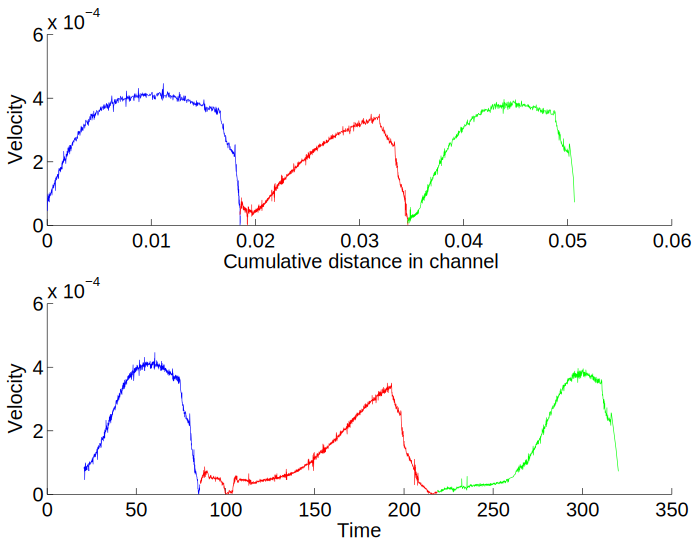
\includegraphics[width=0.7\textwidth]{figures/results/particleA/October_11_Particle_2_run_2_D.pdf}
\end{center}
\caption{The speed (note not the velocity) of the particle A from measurement 1 against cumulative distance in the upper figure and against time in the lower figure.}
\label{fig:particleAspeed}
\end{figure}


\begin{figure}[H]
\begin{center}
\includegraphics[width=0.7\textwidth]{figures/results/particleB/October_1_Particle_4_run_2_D.pdf}
\end{center}
\caption{The speed (note not the velocity) of particle B from measurement 2 against distance in the upper figure and against time in the lower figure. In the plot against time there is an extra dip to 0 at around $t=150$ and $t=400$. This occurs at the end of channel further away from the pump.}
\label{fig:particleB1speed}
\end{figure}


\subsection{Reversals}
In order to show that the dynamics of the particle revert when the flow is reversed we plot the components of $\mathbf{n}$ against distance in the channel. The first reversal from measurement 1 for particle A is seen in Figure \ref{fig:particleAreversegood}. The $n_z$ components are very similar along the entire length of the channel only at the very end does is there a difference larger than the margin of error. The same plot is made from the second reversal from measurement 5 in Figure \ref{fig:particleABadReversal}. Here the particle changes orbit drastically at the reversal while being stable before and after. 

\begin{figure}[H]
\begin{center}
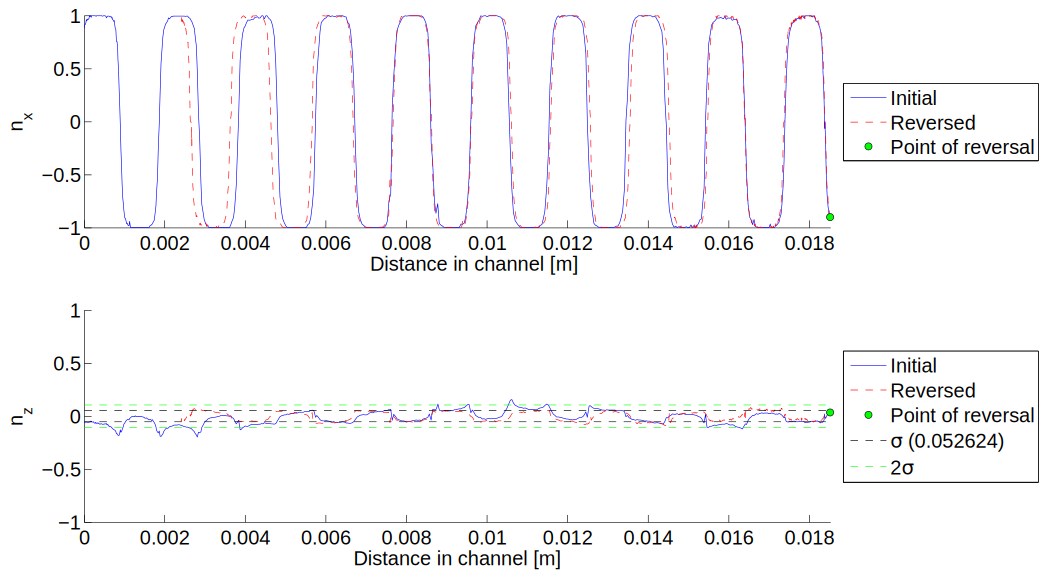
\includegraphics[width=0.7\textwidth]{figures/results/particleA/October_11_Particle_2_run_2_C01.pdf}
\end{center}
\caption{Shows $n_x$ and $n_x$ first and second stretches from Measurement 1, seen in Figure \ref{fig:particleA1} but against the actual position in the channel as opposed to cumulative distance. There is an almost perfect match along the entire channel for $n_x$ and only small disagreement for $n_z$. The dashed lines indicate the error margins for detecting $n_z=0$. This figure is the same as can been seen in Laas\cite{alexanderThesis} Figure 6.21}
\label{fig:particleAreversegood}
\end{figure}

 \begin{figure}[H]
 \centering
 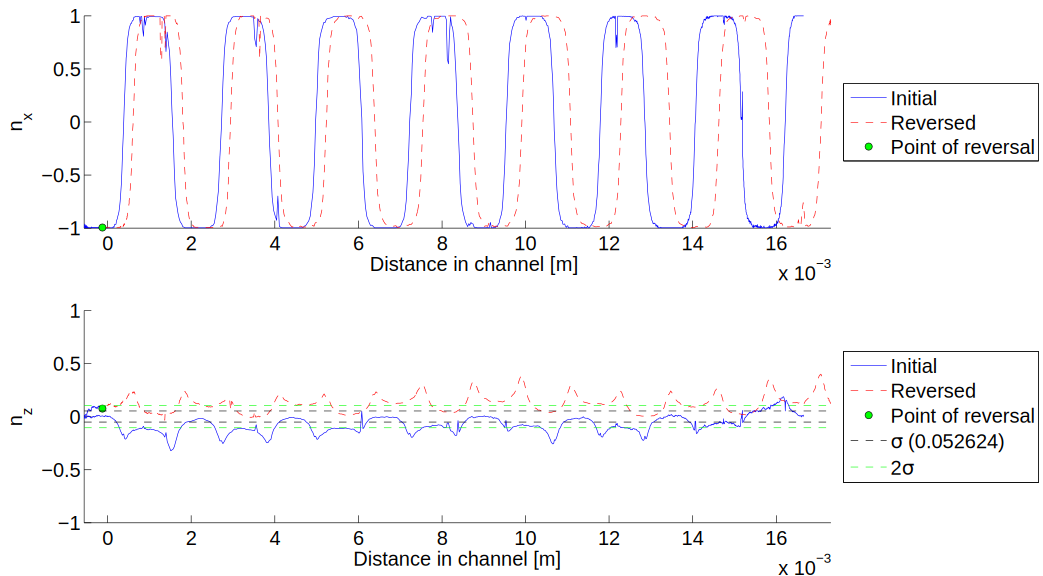
\includegraphics[width=0.8\textwidth]{figures/results/particleA/October_11_Particle_2_run_4_C02.pdf}
 \caption{$n_x$ and $n_z$ from Figure \ref{fig:particleA5} for the second and third stretch plotted against actual distance instead of commutative distance. The reversal occurs at the left and although there is some moderate agreement in $n_x$ the match in $n_z$ is non existant from the very start.}
 \label{fig:particleABadReversal}
 \end{figure}

\section{Match to theoretical orbits}
\subsection{Particle A}
Particle A is approximately \unit[24]{$\mu m$} long so it has a $\lambda$ close to 8 and the closest match for the asymetry is $\epsilon = 0.02$. 

Using the algorithm described in section \ref{sec:matchorbit} we match the data from measurement 1 and 2 for particle A to find the closest matching $\epsilon$ and the best matching orbits. This is shown in Figure \ref{fig:particleAOrbitFit}. We can see that particle A is in a quasi-periodic sign changing orbit during measurement 1, it is matched to the lines indicating A B and C for the first, second and third stretches respectively.  After being shifted by the optical tweezers, particle A followed a periodic orbit during measurement 2. Measurement 2 is matched to the orbits D, E, F and G for the first, second, third and fourth stretches respectively. The stretches that do not have winding numbers listed in the figures had orbits that did not have enough variation in $n_z$ peaks to try to estimate a winding number. 

Note that the orbits shown in Figures \ref{fig:particleAOrbitFit}, \ref{fig:October1Particle4runs2and2Orbits}, and \ref{fig:October1Particle4_runs3and5Orbits} are not the exact orbits matched. The measurements were matched to Poincaré maps with more orbits, but due to aliasing issues of printing such Poincaré maps more sparse Poincaré map are used. Each stretch is printed on the closest matching orbit for $\psi = 0$. The winding numbers are based on the more accurate fit and the better fits are available at \url{http://goo.gl/jgzSXe}. 

\begin{figure}[H]
\begin{center}
\includegraphics[width=\textwidth]{figures/results/orbitmatches/AmapAdded.pdf}
\end{center}
\caption{Black lines show the Poincaré map of the Jeffery's equations for $\lambda = 8$ and $\epsilon = 0.02$. The measured $\lambda$ was $8.2 \pm 0.1$. The orbits of the best fit theoretical fits to measurements are highlighted stretch by stretch. None of the orbits for this particle had any large variations despite being very close to $n_z=0$. The winding numbers are within 50\% of the estimates but both are too low, suggesting that the $\epsilon$ might be too low.}
\label{fig:particleAOrbitFit}
\end{figure}

\subsection{Particle B}

The same procedure is repeated for particle B using the data from measurement 1,2, 3 and 4. To make the graph less cluttered it is split into two figures, Figure \ref{fig:October1Particle4runs2and2Orbits} for measurement 1 and 2 and Figure \ref{fig:October1Particle4_runs3and5Orbits} for measurement 3 and 4. We can see that particle B is in a quasi-periodic sign changing orbit , it is matched to the lines indicating A B and C for the first, second and third stretches respectively.  After being shifted by  the optical tweezer particle A followed a periodic orbit during measurement 2. Measurement 2 is matched to the orbids D, E, F and G for the first, second, third and fourth stretches respectively. 

\begin{figure}[H]
\centering
\includegraphics[width=\textwidth]{figures/results/orbitmatches/Bmap1Added.pdf}
\caption{Black lines show the Poincaré map of the Jeffery's equations for $\lambda = 7$ and $\epsilon=0.04$, the estimate of $\lambda$ from measurement was $6.7 \pm 0.1$. The highlighted orbits are the best fits to the stretches from measurements 1 and 2, A-D from measurement 1 and E-I from measurement 2.}
\label{fig:October1Particle4runs2and2Orbits}
\end{figure}


\begin{figure}[H]
\centering
\includegraphics[width=\textwidth]{figures/results/orbitmatches/Bmap2Added.pdf}
\caption{Black lines show the Poincaré map of the Jeffery's equations for $\lambda = 7$ and $\epsilon = 0.04$. the estimate of $\lambda$ from measurement was $6.7 \pm 0.1$ . The highlighted orbits are the best fits to the stretches from measurements 3 and 4.}
\label{fig:October1Particle4_runs3and5Orbits}
\end{figure}





\chapter{Discussion}
The primary goal of this thesis is to experimentally verify that asymmetric particles in shear flow exhibit different types of motion for different initial conditions, as was predicted by Yarin \emph{et al.}~\cite{Yarin}. To verify that there was no significant amount of noise we look at the reversal of the flow. If the particle retraces its motion it confirms a lack of noise as well as a lack of inertial effects. To estimate the asymmetry $\epsilon$ of the particles we try to match the experimental trajectories over several measurements with theoretical orbits. We also utilize the winding number of quasi-periodic orbits where it can be detected to confirm that the match is valid.

Looking at Figures \ref{fig:October1Particle4_runs3and5Orbits}, \ref{fig:October1Particle4runs2and2Orbits} and \ref{fig:particleAOrbitFit} we find both quasi-periodic and periodic motion as well as all three types of orbits discussed in section \ref{sec:winding}. The winding numbers for the orbits where we can measure it are within $50\%$ of our theoretical predictions. This suggests that we have observed both quasi-periodic orbits and periodic orbits for the same particle two times. We do however have to consider the assumption we make regarding the symmetry difference between the damaged cylinders used experimentally and the flattened spheroids use in theoretical models.

Furthermore our goal was to see that different particles will exhibit different behaviour from the same initial condition based on their asymmetry. Particle A and B exhibit quite different behaviour after the same initial condition $n_z = 0$ with a noticeably lower winding number for particle B and larger fluctuations. However with only 2 particles to compare this and only 1 good measurement for particle A it is still uncertain. 

We have not been able to show a particle exhibiting chaotic motion. This might be due to the relatively small sample of good data or due to the particles being too symmetric. Based on the Poincaré maps in Johansson~\cite{AntonThesis} we see that a larger region of chaotic orbits only appear when $\epsilon \geq 0.2$ and it seems possible based on Figure \ref{fig:particlepictures} and Figure \ref{fig:particlepictures2} that the asymmetry is lower than this for almost all particles. But then it is an open question if we can make that sort of comparison between the asymmetric cylinders and the triaxial particles used in the simulations. 

These results are from a few measurements of two particles, there are many other measurements and other particles that have reversals where there are large differences before and after such as in Figure \ref{fig:particleABadReversal} and Figure \ref{fig:particleA5}. There are four major problems in the data 

\begin{enumerate}
\item Sinking
\item Change in orbit after a reversal
\item Too few flips to clearly estimate winding number
\item Unexplained changes in orbit 
\end{enumerate}

\section{Sinking}
One of the major problems with this setup compared to the previous setup used by Einarsson \emph{et al.} \cite{JonasExperiment} is matching the density of the fluid to that of the particles. Even with a small mismatch of $\unit[0.05]{g/ml}$ we find using eq. (\ref{eq:fallingSphere}) a sinking speed of $= \unit[4.9\cdot10^3 ]{\mu m/s}$. In earlier measurements the pump speed was $\unit[3]{\mu l/minute}$ and the particle were 60\% larger, which meant the sinking occurred more than twice as long and twice as fast which meant it was a larger problem. Even now though it can be noticeably as in longer measurements such as in Figures \ref{fig:particleB2} and \ref{fig:particleB2sinking}.

\section{Reversals where the orbit changes}
Almost every measurement with several stretches have a reversal where the particle noticeably changes orbit. This can been seen in Figures \ref{fig:particleA5}, \ref{fig:particleA4} and \ref{fig:particleB1}. While there is a trend that reversals that do not retrace their orbit occur at he end further from the pump, there are many exceptions to this. There are many cases where the orbit begins to change just as the flow is starting to reverse, such as in Figure \ref{fig:particleA4}. The particle Reynolds number depends on the velocity relative to the particle so a possible culprit could be that reversals occur too rapidly and increase the $Re_p$ such that the $Re_p << 1$ condition from Jeffery \cite{Jeffery} does not hold. We have not been able to draw any clear conclusion and solving issues with reversals would be a tremendous improvement.


\subsection{Possible expansion of the channel}
A possible cause of reversals where the people does not retrace its dynamics when the flow is reversed is that the reversals occur too quickly. A fast reversal could increase the $\Re$ so that we no longer have Stokes flow. To prevent this the reversals are incremental as discussed in Section \ref{sec:exp_setup}. 

Making the reversals slower could solve this issue, but if we look at the speed of the particle A in Figure \ref{fig:particleAspeed} and particle B in Figure \ref{fig:particleB1speed} we see that after a rather 
sharp decline in speed when the reversal starts, the acceleration is slow. Almost all of this acceleration occurs while the pump is 
infusing or withdrawing at a fixed rate. The liquid in the channel accelerating while the pump rate is constant implies that there 
is a noticeable expansion in the channel. To verify this we look again at Figures
\ref{fig:particleAspeed} and \ref{fig:particleB1speed}.

If we have an expanded/contracted channel it should have different effects on different sides of the channel. When the flow is reversed with the particle on the side closer to the pump the impact of the channel should be limited as the only pressure felt by the particle would be built up pressure from the expansion/contraction of the channel. Assuming that the expansion is modest we expect this built up pressure from the channel to be significantly smaller than the one exerted by the pump. So we expect that on this side of the channel the particle reverts quickly.

However when the flow is reversed and the particle is on opposite side of the channel from the pump things are different. Most of the channel feels the pressure difference before the particle so any excess liquid in an expanded channel will slow the reversal of the particle. This would cause a delay where there is no acceleration for some time while after the pump reversed. 

This behaviour is exactly what we see in all speed plots like \ref{fig:particleAspeed} and \ref{fig:particleB1speed}. 
For reversals on the far end of the channel there is a second dip where the particle goes to $\left|v\right|=0$, and in general reversals on the far end are noticeably slow. On the end closer to the pump this 'double dip' never occurs and accelerations are faster, but still slower than if there was no elasticity in the system.

An alternative theory for the delay in reversals would be an offset in the pump, a distance between the syringe handle and the pump holder which would need to be traversed before pumping actually begins, but this would occur at both ends of the channel equally. This does also not explain the long period of acceleration for the particle when the injection rate is constant.

How this impacts the dynamics is not known, however a majority of reversals where the particle does not retrace its orbit occur at the end of the channel close to the pump, which suggests that this extra elasticity in the system might in fact be positive. 

\section{Winding number matching}
Using the score function $\hat{S}$ as described in section \ref{sec:matchorbit} to find the closest matching orbit gives us an estimate of the asymmetry and the orbit of the particle. But it only gives the best fit from a number of different orbits and asymmetries it does not say .  Instead we use the winding number to validate or dismiss a matched orbit and an estimated $\epsilon$. The winding number can only be used for the orbits where $n_z$ changes noticeably, i.e. the quasi-periodic orbits, but these are also the ones of primary interest. 
Figure \ref{fig:windingdifferent} shows that the difference in winding number for the 
same $\theta$ is on the order of a factor 2 between $\epsilon = 0.01$ and $\epsilon = 0.05$ for sign-changing orbits, and 
still quite noticeably different between $\epsilon = 0.05$ and $\epsilon = 0.10$. However the largest difference between different $\epsilon$ is where the change from sign-changing to sign-preserving orbits occur. 

When we look instead at orbits for large $\left| n_z \right|$ such as in Figure 
\ref{fig:October1Particle4runs2and2Orbits} or for $n_z \approx \psi \approx 0$ such as orbit B in Figure 
\ref{fig:particleAOrbitFit} the orbits for different $\epsilon, \lambda$ 
and $i$ are all largely the same. The differences in $n_z$ are too small for us to reliably detect. This creates a problem for 
detecting particles with very small $\epsilon$. For $n_z$ that are very small, we cannot distinguish the orbits for a 
small $\epsilon$ particle with higher $\psi$ orbit for a high $\epsilon$ particle with a low $\psi$ orbit. For higher 
$n_z$ we cannot distinguish straight lines from straight lines. And in the intermediary we are unable to detect a $w 
> 20$, at best finding a sloping $n_z$ which might just be undesired reversals. Particle A has several orbits that 
are matched in the intermediary sign-changing $n_z$ region which we can distinguish from $\epsilon = 0$ but we can not 
estimate the winding number especially well as this measurement is barely half period of the longer period $\theta_1$. 


\section{Unexplained behaviours}
In a number of measurements there are changes in orbit for which we have no explanation. For example in Figure \ref{fig:particleA5} the second reversal is completely sharp, the orbit virtually instantly changes, completely 'forgetting' the previous orbit. Why does this occur with the same particle, the same setup, that produce the excellent reversals in Figure \ref{fig:particleA1}. All conditions we can measure or control are the same and yet the outcome is very different. The only difference is the z coordinate, yet Figure \ref{fig:particleA3} was measured at a similar z and showed very few odd behaviours. 

\section{Width compensation}
The width compensation discussed in Sectinon \ref{sec:width_compensation} does solve the issues the previous algorithm had with 'thick' particles for $n_z$ close to 0. It does still produce small errors for $n_z \neq 0$. However it was discovered that Eq \ref{eq:widthcomp} can be solved explicitly. Given the actual length L of the particle the Euler angle $\theta$ can be solved for at each point after a measurement is complete. This would improve the resolution of peaks and allow for more accurate results.

\section{Goodness of fit}
 The method for matching the data to a theoretical orbit described in \ref{sec:matchorbit} finds the best fit but it is important to know how good of a fit. A flat fitness curve would mean a very small change in the data could lead to a very large change in our matched orbit. To determine the goodness of fit we vary the three parameters separately and find the best fit for the other two parameters. In Figure \ref{fig:asymVariation} we find the best matching orbits for Particle A for asymmetries ranging from 0 to 0.2. We see that there is a clear minima around $\epsilon = 0.02$ implying that it is a good fit.
 
 In Figure \ref{fig:orbitVariation} the match of stretch 1 from measurement 1 of particle A is matched. We use the best matching asymmetry, match for orbits from the center of the pointcare map to the top. For each orbit we find the best starting position (the initial $\psi$). The result is a steady slope down to the correct orbit suggesting that this variable also had a clear best value that was chosen. 
 
 The best In Figure \ref{fig:initVariation} we use the best matching 		asymmetry and orbit for stretch 1 from measurement 1 of particle A, and the starting position (initial $\psi$) is varied over 1 full period. The relatively flat slope suggests that this parameter while certainly improving the fit slightly is not as important as the other two parameters. 
 
 \begin{figure}[H]
 \begin{center}
 \includegraphics[width=0.7\textwidth]{figures/results/particleA/A_assymVariation.pdf}
 \end{center}
 \caption{We see how the difference between the theoretical $n_z$ and all the measured  $\widetilde{n_z}$ for all measurements of particle A for different asymmetries $\epsilon$. For each asymmetry we find the orbit and the initial $\psi$ with the smallest distance for each stretch. We see that there is a clear minima around $\epsilon = 0.02$}
 \label{fig:asymVariation}
 \end{figure}
 
 \begin{figure}[H]
 \begin{center}
 \includegraphics[width=0.7\textwidth]{figures/results/particleA/A_orbitVariation.pdf}
 \end{center}
 \caption{The difference between the theoretical $n_z$ and the measured $\widetilde{n_z}$ for the first stretch of the measurement 1 for particle A (seen in figure \ref{fig:particleA1})with the best asymmetry for different orbits. .}
 \label{fig:orbitVariation}
 \end{figure}
 
 
 \begin{figure}[H]
 \begin{center}
 \includegraphics[width=0.7\textwidth]{figures/results/particleA/A_posVariation.pdf}
 \end{center}
 \caption{The difference between the theoretical $n_z$ and the measured $\widetilde{n_z}$ for the first stretch of the first measurement for particle A. The best orbit and best asymmetry are chosen, but different initial conditions are tested. }
 \label{fig:initVariation}
 \end{figure}
 



\chapter{Conclusion}
The conclusion is that we found something.


%\section{$\mathbf{\lambda}$ of about 6}
%These are the particles with a $\lambda = 6 \pm 0.5$
%\subsection{Particle 1}

\begin{figure}[H]
\centering
\includegraphics[width=0.8\textwidth]{Images/Particle 1/Particle1.pdf}
\caption{Particle 1: $ \lambda: 6.1591$Depth: 160 out of $200 \mu $ m}
\end{figure}

\begin{figure}[H]

\centering

\includegraphics[width=0.8\textwidth]{Images/Particle 1/Stretch1.pdf}

\end{figure}

\begin{figure}[H]

\centering

\includegraphics[width=0.8\textwidth]{Images/Particle 1/Stretch2.pdf}

\end{figure}

\subsection{Particle 4}

\begin{figure}[H]
\centering
\includegraphics[width=0.8\textwidth]{Images/Particle 4/Particle4.pdf}
\caption{Particle 4: At around 10 minutes, pretty big "jump" in channel flow. $ \lambda: 12.7745$Depth: 140 out of $200 \mu $ m}
\end{figure}

\begin{figure}[H]
\centering
\includegraphics[width=0.8\textwidth]{Images/Particle 4/Stretch1.pdf}
\end{figure}


\begin{figure}[H]
\centering
\includegraphics[width=0.8\textwidth]{Images/Particle 4/Stretch2.pdf}
\end{figure}


\subsection{Particle 11}

\begin{figure}[H]
\centering
\includegraphics[width=0.8\textwidth]{Images/Particle 11/Particle11.pdf}
\caption{Particle 11: At around 7:03, possible interaction with dirt in channel. $ \lambda: 5.9638$Depth: 180 out of $200 \mu $ m}
\end{figure}

\begin{figure}[H]
\centering
\includegraphics[width=0.8\textwidth]{Images/Particle 11/Stretch1.pdf}
\end{figure}

\begin{figure}[H]
\centering
\includegraphics[width=0.8\textwidth]{Images/Particle 11/Stretch2.pdf}
\end{figure}


\subsection{Particle 13}
\begin{figure}[H]
\centering
\includegraphics[width=0.8\textwidth]{Images/Particle 13/Particle13.pdf}
\caption{Particle 13: At around 4:15 there is a big jump in the flow at reversal. $ \lambda: 5.5457$Depth: 140 out of $200 \mu $ m}
\end{figure}

\begin{figure}[H]
\centering
\includegraphics[width=0.8\textwidth]{Images/Particle 13/Stretch1.pdf}
\end{figure}


\subsection{Particle 16}
\begin{figure}[H]
\centering
\includegraphics[width=0.8\textwidth]{Images/Particle 16/Particle16.pdf}
\caption{Particle 16: $ \lambda: 6.2917$Depth: 120 out of $200 \mu $ m}
\end{figure}

\begin{figure}[H]

\centering

\includegraphics[width=0.8\textwidth]{Images/Particle 16/Stretch1.pdf}

\end{figure}

\begin{figure}[H]

\centering

\includegraphics[width=0.8\textwidth]{Images/Particle 16/Stretch2.pdf}

\end{figure}



\subsection{Particle 22}

\begin{figure}[H]


\centering
\includegraphics[width=0.8\textwidth]{Images/Particle 22/Particle22.pdf}
\caption{Particle 22: $ \lambda: 11.6767$Depth: 160 out of $200 \mu $ m}

\end{figure}

\begin{figure}[H]

\centering

\includegraphics[width=0.8\textwidth]{Images/Particle 22/Stretch1.pdf}

\end{figure}

\begin{figure}[H]

\centering

\includegraphics[width=0.8\textwidth]{Images/Particle 22/Stretch2.pdf}

\end{figure}

\subsection{Particle 23}

\begin{figure}[H]
\centering
\includegraphics[width=0.8\textwidth]{Images/Particle 23/Particle23.pdf}
\caption{Particle 23: $ \lambda: 5.6106$Depth: 80 out of $200 \mu $ m}
\end{figure}

\begin{figure}[H]
\centering
\includegraphics[width=0.8\textwidth]{Images/Particle 23/Stretch1.pdf}
\end{figure}




%
%\section{$\mathbf{\lambda}$ of about 6}
%These are the particles with a $\lambda = 7 \pm 0.5$
%\subsection{Particle 2}

\begin{figure}[ H]

\caption{Particle 2: $ \lambda: 13.9227$Depth: 30 out of $200 \mu $ m}

\centering

\includegraphics[width=0.8\textwidth]{Images/Particle 2/Particle2.pdf}

\end{figure}

\begin{figure}[ H]

\centering

\includegraphics[width=0.8\textwidth]{Images/Particle 2/Stretch1.pdf}

\end{figure}

\begin{figure}[ H]

\centering

\includegraphics[width=0.8\textwidth]{Images/Particle 2/Stretch2.pdf}

\end{figure}

\begin{figure}[ H]

\centering

\includegraphics[width=0.8\textwidth]{Images/Particle 2/Stretch3.pdf}

\end{figure}

\begin{figure}[ H]

\centering

\includegraphics[width=0.8\textwidth]{Images/Particle 2/Stretch4.pdf}

\end{figure}

\begin{figure}[ H]

\centering

\includegraphics[width=0.8\textwidth]{Images/Particle 2/Stretch5.pdf}

\end{figure}

\begin{figure}[ H]

\centering

\includegraphics[width=0.8\textwidth]{Images/Particle 2/Stretch6.pdf}

\end{figure}


\subsection{Particle 7}

\begin{figure}[ H]

\caption{Particle 7: $ \lambda: 27.4694$Depth: 20 out of $200 \mu $ m}

\centering

\includegraphics[width=0.8\textwidth]{Images/Particle 7/Particle7.pdf}

\end{figure}


\subsection{Particle 18}

\begin{figure}[ H]

\caption{Particle 18: Unclear. There are several possible interactions around 6 minutes but neither is all too clear. Also the second turn is overall quite jumpy$ \lambda: 14.3568$Depth: 20 out of $200 \mu $ m}

\centering

\includegraphics[width=0.8\textwidth]{Images/Particle 18/Particle18.pdf}

\end{figure}

\begin{figure}[ H]

\centering

\includegraphics[width=0.8\textwidth]{Images/Particle 18/Stretch1.pdf}

\end{figure}

\begin{figure}[ H]

\centering

\includegraphics[width=0.8\textwidth]{Images/Particle 18/Stretch2.pdf}

\end{figure}


\subsection{Particle 19}

\begin{figure}[ H]

\caption{Particle 19: At around 0:50 there is an uneven vertical flow "surging" the particle down. $ \lambda: 13.795$Depth: 120 out of $200 \mu $ m}

\centering

\includegraphics[width=0.8\textwidth]{Images/Particle 19/Particle19.pdf}

\end{figure}

\begin{figure}[ H]

\centering

\includegraphics[width=0.8\textwidth]{Images/Particle 19/Stretch1.pdf}

\end{figure}

\begin{figure}[ H]

\centering

\includegraphics[width=0.8\textwidth]{Images/Particle 19/Stretch2.pdf}

\end{figure}



 


\subsection{Particle 20}

\begin{figure}[ H]

\caption{Particle 20: At 5:22 collides with large "debris" on channel floor. $ \lambda: 13.5864$Depth: 150 out of $200 \mu $ m}

\centering

\includegraphics[width=0.8\textwidth]{Images/Particle 20/Particle20.pdf}

\end{figure}

\begin{figure}[ H]

\centering

\includegraphics[width=0.8\textwidth]{Images/Particle 20/Stretch1.pdf}

\end{figure}



\subsection{Particle 24}

\begin{figure}[ H]

\caption{Particle 24: $ \lambda: 14.3715$Depth: 60 out of $200 \mu $ m}

\centering

\includegraphics[width=0.8\textwidth]{Images/Particle 24/Particle24.pdf}

\end{figure}

\begin{figure}[ H]

\centering

\includegraphics[width=0.8\textwidth]{Images/Particle 24/Stretch1.pdf}

\end{figure}

\begin{figure}[ H]

\centering

\includegraphics[width=0.8\textwidth]{Images/Particle 24/Stretch2.pdf}

\end{figure}

%
%\section{Other particles}
%\subsection{Particle 3}

\begin{figure}[H]

\includegraphics[width=0.8\textwidth]{Images/Particle 3/Particle3.pdf}

\caption{Particle 3:  $ \lambda: 19.5489$ Depth: 140 out of $200 \mu $ m}

\centering

\end{figure}

\begin{figure}[H]

\centering

\includegraphics[width=0.8\textwidth]{Images/Particle 3/Stretch1.pdf}

\end{figure}


\subsection{Particle 5}

\begin{figure}[H]

\includegraphics[width=0.8\textwidth]{Images/Particle 5/Particle5.pdf}

\caption{Particle 5:  $ \lambda: 15.2445$ Depth: 160 out of $200 \mu $ m}

\centering

\end{figure}

\begin{figure}[H]

\centering

\includegraphics[width=0.8\textwidth]{Images/Particle 5/Stretch1.pdf}

\end{figure}

\begin{figure}[H]

\centering

\includegraphics[width=0.8\textwidth]{Images/Particle 5/Stretch2.pdf}

\end{figure}


\subsection{Particle 6}

\begin{figure}[H]
\includegraphics[width=0.8\textwidth]{Images/Particle 6/Particle6.pdf}
\caption{Particle 6:  $ \lambda: 17.3351$ Depth: 150 out of $200 \mu $ m}
\centering

\end{figure}

\begin{figure}[H]

\centering

\includegraphics[width=0.8\textwidth]{Images/Particle 6/Stretch1.pdf}

\end{figure}

\begin{figure}[H]

\centering

\includegraphics[width=0.8\textwidth]{Images/Particle 6/Stretch2.pdf}

\end{figure}

\subsection{Particle 8}

\begin{figure}[H]

\includegraphics[width=0.8\textwidth]{Images/Particle 8/Particle8.pdf}

\caption{Particle 8:  $ \lambda: 36.1074$ Depth: 120 out of $200 \mu $ m}

\centering

\end{figure}

\subsection{Particle 9}

\begin{figure}[H]

\includegraphics[width=0.8\textwidth]{Images/Particle 9/Particle9.pdf}

\caption{Particle 9:  $ \lambda: 7.5902$ Depth: 160 out of $200 \mu $ m}

\centering

\end{figure}

\subsection{Particle 10}

\begin{figure}[H]

\includegraphics[width=0.8\textwidth]{Images/Particle 10/Particle10.pdf}

\caption{Particle 10:  $ \lambda: 8.6589$ Depth: 60 out of $200 \mu $ m}

\centering

\end{figure}

\begin{figure}[H]

\centering

\includegraphics[width=0.8\textwidth]{Images/Particle 10/Stretch1.pdf}

\end{figure}

\subsection{Particle 12}

\begin{figure}[H]

\includegraphics[width=0.8\textwidth]{Images/Particle 12/Particle12.pdf}

\caption{Particle 12:  $ \lambda: 8.1961$ Depth: 180 out of $200 \mu $ m}

\centering

\end{figure}

\begin{figure}[H]

\centering

\includegraphics[width=0.8\textwidth]{Images/Particle 12/Stretch1.pdf}

\end{figure}


\subsection{Particle 15}

\begin{figure}[H]

\includegraphics[width=0.8\textwidth]{Images/Particle 15/Particle15.pdf}

\caption{Particle 15:  $ \lambda: 7.7306$ Depth: 120 out of $200 \mu $ m}

\centering

\end{figure}

\begin{figure}[H]

\centering

\includegraphics[width=0.8\textwidth]{Images/Particle 15/Stretch1.pdf}

\end{figure}

\begin{figure}[H]

\centering

\includegraphics[width=0.8\textwidth]{Images/Particle 15/Stretch2.pdf}

\end{figure}


\subsection{Particle 17}

\begin{figure}[H]

\includegraphics[width=0.8\textwidth]{Images/Particle 17/Particle17.pdf}

\caption{Particle 17:  $ \lambda: 7.6562$ Depth: 180 out of $200 \mu $ m}

\centering

\end{figure}

\begin{figure}[H]

\centering

\includegraphics[width=0.8\textwidth]{Images/Particle 17/Stretch1.pdf}

\end{figure}

\begin{figure}[H]

\centering

\includegraphics[width=0.8\textwidth]{Images/Particle 17/Stretch2.pdf}

\end{figure}

\subsection{Particle 21}

\begin{figure}[H]

\includegraphics[width=0.8\textwidth]{Images/Particle 21/Particle21.pdf}

\caption{Particle 21:  $ \lambda: 9.6776$ Depth: 60 out of $200 \mu $ m}

\centering

\end{figure}

\begin{figure}[H]

\centering

\includegraphics[width=0.8\textwidth]{Images/Particle 21/Stretch1.pdf}

\end{figure}

\begin{figure}[H]

\centering

\includegraphics[width=0.8\textwidth]{Images/Particle 21/Stretch2.pdf}

\end{figure}

\bibliography{bibliography}
\bibliographystyle{plain}
\end{document}     

% This should not be a chapter but a section of the experimental setup. Maybe a section of 
% that should be improvements and I can include the Automated tracking can be part of that
% I should also ask Dag if it's reasonable to include a section of attempted improvements, as
% a guideline to anyone who tris to replicate the experiment both about what can be done (for inspiration)
% but then as a caution that while you may try this it did not work for us

 % %%sTODO:
%READ UP ON THE EFFICIENCY OF THE CANNY EDGE DETECTION
%TAKE AN IMAGE OF THE STATIC NOISE REDUCTION (DOES IT ACTUALLY WORK?!)
%GET AN IMAGE OF BEFORE AND AFTER SMOOTHING, PREFERABLY INCLUDE A CANNY EDGE DETECTION OF BOTH 
%WRITE ABOUT THE TIME IT TAKES TO DO VARIOUS STUFFS (IS THIS NEEDED?)
%%
%JEFFREY ORBIT STUFF:
%mention the aspect ratio and the importance is has on the period time
%
%DATA ANALYSIS STUFF:
%Add citation for ellipse fit
%Make graph of mode of lengths?
%Add cite to anton for a bunch of stuff since i am stealing. 
%
%
%EXPERIMENTAL SETUP STUFF:
%Include the distribution of lengths, either meassured or from nippon
%Make an image of the correction for width and !!!discuss it. !!!


%\section{Particle tracking}
%\subsection{Noise Reduction}
The first step in tracking a particle is to correctly identify it in the image given. To do this we want to eliminate as much noise from the image as we can. The first type of noise we will eliminate is static noise, this is noise present in every image and results from dirt or scratches on the lens of the camera or microscope. 
The easiest solution to such noise would of course be to clean the instruments, but despite numerous attempts of carefully cleaning every surface a noticeable of static noise would always remain. 

This means one must use algorithmic noise reduction methods to remove this noise. The method employed is a simple averaging that takes N pictures at different positions in the channel to generate an average image where any particular features of the channel would disappear and only the static noise remain. This can be seen in figure STATIC NOISE REDUCTION IMAGE,


\subsection{Canny Edge Detection}
The Canny Edge invented by John Canny in his 2011 paper the canny of cane detection is generally considered the most advanced and best performing edge detection of the simple filter functions. 
Without going in to the finer details, given an image matrix $\mathbf{I}$ where each value corresponds to the light intensity $i_{x,y}$of that pixel at index $x,y$ the Canny edge detector will try to find the cohesive pixels $E = \{e_1, e_2... e_n\}$ where there is a noticeable change in intensity. In other words, what we call an "edge" an image. 

This is accomplished in two steps. First a Sobel Filter edge image is computed by looking at the change in intensity at every pixel from 3 possible directions and averaging these. 

S = MATHEMATICS OF SOBEL

We then consider a Then, a pixel 

$p_{x,y} \in E \text{if} S(x,y) > T_{high}$

where $T_{high}$ is a predetermined threshold value. 

Secondly we recursively check all pixels neighbouring an edge

MATH?

 if they are higher than some threshold value $T_low$. if they are, they are also considered part of the edge. This is repeated until no more pixels are added. An image illustrating this process can be seen in figure FIG. The benefit of the Canny edge detection over the simpler Sobel is that it is much easier to detect cohesive objects that vary in intensity without getting a lot of other noise in the image. The only real drawback of the Canny Edge detection is the computation time, and thus the implementation from the Open Computer Vision (OCV) was used, as this is a heavily optimized routine written in C++ with real time uses in mind. Thanks to this the computing for the Canny Edge of a 260x260 Image takes about X ms and thus is of little importance in the overall time per frame.

After noise reduction the Canny Edge Detection is used to find the most significant edges in the image. 

\subsection{Contour detection and selection}

Once an edge image has been generated, the OCV package has another useful function, \texttt{Contours} which returns a list of every contiguous group of edge pixels. If we have chosen the threshold values to the edge detection correctly, this should include the particle or a good approximation of it. 

In order to find the correct contour, a few techniques are used to find the correct contour.

First particles whose total size is less than some minimum value, $ n_{min}$ or larger than some maximum value $n_{max}$ are ignored. Then the position $pP_i$ of each contour $C_i={p_1,p_2...p_n}$ is calculated as the average pixel position

\[
P_i = \sum_{j}^n p_j/n
\]
This position is compared to the expected position of the Kalman filter, which the very first frame is the middle position. 

Finally a 'thinness value' is calculated according to eq \ref{eq:thinness}

\begin{equation}\label{eq:thinness}
w_{thin}\left(\frac{ n}{d_{max}^2}\right)^2
\end{equation}. 
where $w_{thin}$ is a weighting constant, $n$ is the number of pixels in the contour and $d_{max}$ is the longest distance between two pixels in the 
where I am not really sure I should do this now that I have so few particles, but I do it none the less!

\subsection{Stabilizing the tracking}
Once a state estimation has been made, we want to adjust the speed of the step engine to, as best as possible, match that of the particle. This is done by looking both the position and velocity of the particle and going through the conditional statements shown in figure CONDITIONAL CORRECTION VECTOR. 

The goal is to limit the amount of corrections made, as changing the velocity is rather time intensive as discussed in section \ref{sec:time considerations}, as well as keeping the particle stable. There is also no point in trying to completely eliminate movement
% % About how to choose the correction vector and communicate with the step engine

\subsection{Time Considerations}\label{sec:time considerations}
A higher FPS will allow the particle detection to be better, improve the position saving and allow the particle tracking to be more stable as well. So maximizing the FPS, ie reducing the computational time of each task, is a clear goal for a good automated tracking. A list of the different tasks and their average execution times can be seen in table \ref{tab:benchmarks}

\begin{table}[H]
 \begin{tabular}{l | c | c } 
 Task  			&  Average time & Std deviation \\
 Capture screen & 1000 			& 200 \\
 Find edges 	& 200			& 20 \\
 \end{tabular}
 \caption{}
 \label{tab:benchmarks}
\end{table}

We can clearly see that FPS is limited primarily by three routines: The screen capture routine, the change velocity routine and finally the save position routine. The first and last are unavoidable and must be done every frame by definition if we are interested in knowing the particles position as well as possible. This means we simply want to use the velocity correction as little as possible. Since the time constraint is in the communication with the step engine, there is not any optimization to be done here, at least not within the scope is this thesis. 


%\section{Kalman Filter}
%	When the particle is at constant motion in the channel the equations of motion give us
	\begin{equation}
	\left[
	\begin{array}{c}
	  x_n	 \\
	 	  v_{x,n} \\ 
	  y_n	 \\
	  v_{y,n} 
	\end{array} 
	\right]
	 =
	 \begin{bmatrix}
	  x_{n-1} & + v_{x,n-1} \\
	  v_{x,n-1}       & ...		 \\
	  y_{n-1} &+v_{y,n-1}  \\
	  v_{y,n-1}       &		\\
	 \end{bmatrix}
	+
	\left[
	\begin{array}{c}
	0 \\
	c_{xn} \\
	0 \\
	c_{yn}
	\end{array}
	\right]
	%	x_n \right] = \left[ x_{n-1}+ v_{n+1} \right]\\
	%	v_{xn}
		y_n
		v_{yn}
	\end{equation}
	
	We can rewrite this in matrix form as
	
	\begin{equation}
	\left[
	 \begin{array}{c}
	 x_{n} \\
	 v_{x,n}\\
	 y_{n}\\
	 v_{y,n}
	 \end{array}
	 \right]
	 =
	 \begin{bmatrix}
	  1 & 	\Delta t & 	0 & 	0 \\
	  0 & 	1 & 	0 & 		0 \\
	  0 & 	0 & 	1 & \Delta t  \\
	  0 & 	0 & 	0 & 		1 \\
	 \end{bmatrix}
	 \cdot
	 \left[
	 \begin{array}{c}
	 x_{n-1} \\
	 v_{x,n-1}\\
	 y_{n-1}\\
	 v_{y,n-1}
	 \end{array}
	\right]
	 +
	 \begin{bmatrix}
	   0 & 	0 & 	0 & 	0 \\
	   0 & 	1 &		0 & 	0 \\
	   0 & 	0 & 	0 &    	0 \\
	   0 & 	0 & 	0 & 	1 \\
	  \end{bmatrix}
	  \cdot
	  \begin{array}{c}
	  0 \\
	  c_{x,n-1} \\
	  0 \\
	  c_{y,n-1}
	  \end{array}
	\end{equation}
	
	Now if we want to transform this to the measured data we have to simply multiply by a constant pixel-to-meter constant, which has been meassured to be around $1/940=1.06\cdot 10^{-3}$
	
	\begin{equation}
	Q = 
	 \begin{bmatrix}
	  0 & 	0 & 	0 & 	0 \\
	   0 & 	1 &		0 & 	0 \\
	   0 & 	0 & 	0 &    	0 \\
	   0 & 	0 & 	0 & 	1 \\
	  \end{bmatrix}
	\end{equation}
	
	Which we can easily re-write as a Kalman filter 
	\begin{equation}
	\hat{\mathbf{x}}_{n} = \mathbf{A}_n\mathbf{x_{n-1}} + \mathbf{B}_n \mathbf{u}_n + \mathbf{w}_n
	\end{equation}
	\begin{equation}
	\hat{\mathbf{P}}_n = \mathbf{F}_n \mathbf{P}_{n-1} \mathbf{F}^{T}_{n} + \mathbf{Q}_n
	\end{equation}
	with 
	\begin{eqnarray}
	\mathbf{x}_n &= 
	\left[
	x_n 
	v_{x,n} 
	y_n 
	v_{y,n}
	\right]^T \\
	\mathbf{A} &= 
	\begin{bmatrix}
	  1 & 	\Delta t & 	0 & 	0 \\
	  0 & 	1 & 	0 & 		0 \\
	  0 & 	0 & 	1 & \Delta t  \\
	  0 & 	0 & 	0 & 		1 \\
	\end{bmatrix} \\
	\mathbf{B}_n &= 
	 \begin{bmatrix}
	   0 & 	0 & 	0 & 	0 \\
	   0 & 	1 &		0 & 	0 \\
	   0 & 	0 & 	0 &    	0 \\
	   0 & 	0 & 	0 & 	1 \\
	  \end{bmatrix}
	\\
	\mathbf{u}_n &=
	\left[
	  \begin{array}{c}
	  0 \\
	  c_{x,n-1} \\
	  0 \\
	  c_{y,n-1}
	  \end{array}
	  \right] 
	\end{eqnarray}
	
	and we add the update part as
	\begin{eqnarray}
	&\mathbf{K}_n = \hat{\mathbf{P}}_n \mathbf{H}^T_n(\mathbf{H}_n \hat{\mathbf{P}}_n \mathbf{H}^T_n	) \\
	&\mathbf{x_n} = \hat{\mathbf{x}}_n + \mathbf{K}_n(\mathbf{y} - \mathbf{H}_n\hat{\mathbf{x}}_n) \\
	&\mathbf{P}   = (\mathbf{I} - \mathbf{K}_n\mathbf{H}_n)\hat{\mathbf{P}}_n
	\end{eqnarray}
	
	
	
	
	

